% \iffalse meta-comment
% ======================================================================
% contract.dtx
% Copyright (c) Markus Kohm, 2007-2023
%
% This file is part of the LaTeX2e KOMA-Script bundle.
%
% This work may be distributed and/or modified under the conditions of
% the LaTeX Project Public License, version 1.3c of the license.
% The latest version of this license is in
%   http://www.latex-project.org/lppl.txt
% and version 1.3c or later is part of all distributions of LaTeX
% version 2005/12/01 or later and of this work.
%
% This work has the LPPL maintenance status "author-maintained".
%
% The Current Maintainer and author of this work is Markus Kohm.
%
% This work consists of the files listed in MANIFEST.md.
% ======================================================================
%<identify>%%% --- docstrip run: identify ---
%<doc>%%% --- docstrip run: doc ---
%<init>%%% --- docstrip run: init ---
%<options>%%% --- docstrip run: options ---
%<postoptions>%%% --- docstrip run: postoptions ---
%<body>%%% --- docstrip run: body ---
%<final>%%% --- docstrip run: final ---
%<*dtx>
\expandafter\ifx\csname ProvidesFile\endcsname\relax
  \def\ProvidesFile#1[#2]{}
\fi
\ProvidesFile{contract.dtx}[%
%</dtx>
%<package&identify>\NeedsTeXFormat{LaTeX2e}[1995/06/01]
%<package&identify>\ProvidesPackage{contract}[%
%<doc&identify&en>\ProvidesFile{contract-en.tex}[%
%<doc&identify&de>\ProvidesFile{contract-de.tex}[%
%<*dtx|(package&identify)>
  2023-10-10 v0.0.1
%<doc&identify>  documentation of
%<*dtx>
  source of
%</dtx>
  package for jurists
]
%</dtx|(package&identify)>
%<*dtx>
\ifx\documentclass\undefined
%</dtx>
%<*ins>
  \input docstrip.tex
  \generate{\usepreamble\defaultpreamble
%    \file{contract.ins}{%
%      \from{contract.dtx}{ins}%
%    }%
    \file{contract.sty}{%
      \from{contract.dtx}{package,identify}%
      \from{contract.dtx}{package,init}%
      \from{contract.dtx}{package,options}%
      \from{contract.dtx}{package,postoptions}%
      \from{contract.dtx}{package,body}%
      \from{contract.dtx}{package,final}%
    }%
  }%
%</ins>
%<*dtx>
\else
  \let\endbatchfile\relax
\fi
%</dtx>
%<*ins>
\endbatchfile
%</ins>
%<*dtx>
\documentclass[USenglish,ngerman]{koma-script-source-doc}
\usepackage[T1]{fontenc}
\usepackage{lmodern}
\usepackage[main=USenglish]{babel}
\usepackage{graphicx}
\usepackage[colorize]{scrguide-listings}
\usepackage{scrguide-doclink}
\usepackage{booktabs}
\usepackage{csquotes}
\usepackage[style=alphabetic]{biblatex}
\begin{filecontents}{\jobname.bib}
@online{pkg:koma-script,
  author={Markus Kohm},
  version={3.41},
  date={2023-07-07},
  title={{\KOMAScript} --- A bundle of versatile classes and packages},
  url={https://ctan.org/pkg/koma-script},
  urldate={2023-07-14},
  note={The \KOMAScript{} bundle provides replacements for the \cls*{article},
        \cls*{report}, and \cls*{book} classes with emphasis on typography and
        versatility. There is also a letter class.},
}
@manual{pkg:koma-script:manual:de,
  author={Markus Kohm},
  date={2023-06-16},
  title={{\KOMAScript}},
  subtitle={Die Anleitung},
  url={http://mirrors.ctan.org/macros/latex/contrib/koma-script/scrguide-de.pdf}
,
  urldate={2023-07-04},
}
@manual{pkg:koma-script:manual:en,
  author={Markus Kohm},
  date={2023-06-16},
  title={{\KOMAScript}},
  subtitle={The Guide},
  url={http://mirrors.ctan.org/macros/latex/contrib/koma-script/scrguide-en.pdf},
  urldate={2023-07-14},
}
\end{filecontents}
\addbibresource{\jobname.bib}
\setcounter{StandardModuleDepth}{2}
\newcommand*{\Index}{\index}
\newcommand*{\LabelBase}{contract}
\newcommand*{\seclabel}[1]{\label{sec:\LabelBase.#1}}
\newcommand*{\PValue}{\texttt}
\newcommand*{\PName}{\meta}
\newcommand*{\Option}{\opt}
\newcommand*{\OptionValue}[2]{\texttt{#1=\linebreak[2]#2}}
\newcommand*{\OptionVName}[2]{\texttt{#1=\linebreak[2]\meta{#2}}}
\newcommand*{\Length}{\len}
\newcommand*{\Counter}{\cnt}
\newcommand*{\BeginIndexGroup}{}
\newcommand*{\BeginIndex}[2]{}
\newcommand*{\EndIndex}[2]{}
\newcommand*{\EndIndexGroup}{}
\newcommand*{\Class}{\cls}
\newcommand*{\PageStyle}{\pstyle}
\newcommand*{\IndexCounter}{\SpecialCounterIndex}
\newcommand*{\IndexCmd}{\SpecialCommandIndex}
\newcommand*{\IndexOption}{\SpecialOptionIndex}
\newcommand*{\IndexPackage}[1]{}
\newcommand*{\IndexFontElement}{\SpecialKOMAfontIndex}
\newcommand*{\textKValue}{\optvalue}
\newcommand*{\SeeNote}[1]{\nobreak}
\newcommand*{\Macro}{\cs}
\newcommand*{\Environment}{\env}
\newcommand*{\OParameter}{\oarg}
\newcommand*{\Parameter}{\marg}
\newcommand*{\PParameter}[1]{\texttt{\{#1\}}}
\newcommand*{\POParameter}[1]{\texttt{[#1]}}
\newcommand*{\LabelFontElement}[1]{%
  \DescribeKOMAfont[noprint]{#1}%
  {\def\meta##1{/##1/}\phantomsection\label{desc:\LabelBase.fontelement.#1}}}
\newcommand*{\FontElement}{\fnt}
\newenvironment{desctabular}{%
  \newcommand{\entry}[2]{\item[{##1}:]##2}%
  \begin{description}
}{%
  \end{description}
}
\newenvironment{desclist}{%
  \newcommand*{\desccaption}[2]{%
    \par
    \vspace{5\baselineskip}\pagebreak[2]\vspace{-5\baselineskip}\nopagebreak
    \captionof{table}{##1}\nopagebreak
    \begin{desctabular}
  }%
}{%
  \end{desctabular}
}
\newcommand*{\OptionValueRef}[3]{\OptionValue{#2}{#3}}  
\makeatletter
\newenvironment{Declaration}{%
  \begin{lrbox}{\@tempboxa}
}{\end{lrbox}}
\newcommand*{\DescRef}[1]{\@DescRef#1\@nil}
\def\@DescRef #1.#2.#3\@nil{%
  \Ifstr{#2}{counter}{\cnt{#3}}{%
    \Ifstr{#2}{cmd}{\cs{#3}}{%
      \Ifstr{#2}{env}{\env{#3}}{%
        \Ifstr{#2}{option}{\opt{#3}}{%
          \undefined
        }}}}%
}
\makeatother
\newcommand*{\important}[2][]{}
\newcommand*{\textnote}[1]{}
\newenvironment{Example}{%
  \lstset{belowskip=0pt plus 1pt minus .5pt}%
  \labeling{{\usekomafont{disposition}\Examplename:}}
  \item[{\usekomafont{disposition}\Examplename:}]%
}{%
  \endlabeling
}
\newcaptionname{USenglish}{\Examplename}{Example}
\newcaptionname{ngerman}{\Examplename}{Beispiel}
\newcommand{\iffree}[2]{#1}
\DeclareTOCStyleEntry[dynnumwidth,dynindent]{section}{section}
\DeclareTOCStyleEntries[dynnumwidth,dynindent]{subsection}{subsection,subsubsection}
\usepackage{hyperref}
\DeclareLinkFallback{Macro}{arabic}
  {https://en.wikibooks.org/wiki/LaTeX/Counters#Counter_style}
\DeclareLinkFallback{Macro}{begin}
  {https://en.wikibooks.org/wiki/LaTeX/Basics#LaTeX_environments}
\DeclareLinkFallback{Macro}{bfseries}
  {https://en.wikibooks.org/wiki/LaTeX/Fonts#Font_styles}
\DeclareLinkFallback{Macro}{end}
  {https://en.wikibooks.org/wiki/LaTeX/Basics#LaTeX_environments}
\DeclareLinkFallback{Macro}{refstepcounter}
  {https://en.wikibooks.org/wiki/LaTeX/Counters#Counter_manipulation}
\DeclareLinkFallback{Macro}{sffamily}
  {https://en.wikibooks.org/wiki/LaTeX/Fonts#Font_styles}
  
\DeclareLinkFallback{Macro}{defineshorthand}
  {file:../babel/babel.pdf#subsection.1.10}  
\DeclareLinkFallback{Macro}{useshorthand}
  {file:../babel/babel.pdf#subsection.1.10}  
  
\DeclareLinkFallback{Macro}{setkeys}
  {file:../graphics/keyval.pdf#section.3}

\DeclareLinkFallback{Macro}{documentclass}
  {file:../lshort-english/lshort.pdf#12}
\DeclareLinkFallback{Macro}{dots}
  {file:../lshort-english/lshort.pdf#a7}
\DeclareLinkFallback{Macro}{label}
  {file:../lshort-english/lshort.pdf#2b}
\DeclareLinkFallback{Macro}{large}
  {file:../lshort-english/lshort.pdf#b3}
\DeclareLinkFallback{Macro}{pageref}
  {file:../lshort-english/lshort.pdf#2b}
\DeclareLinkFallback{Macro}{paragraph}
  {file:../lshort-english/lshort.pdf#2a}
\DeclareLinkFallback{Macro}{ref}
  {file:../lshort-english/lshort.pdf#2b}
\DeclareLinkFallback{Macro}{section}
  {file:../lshort-english/lshort.pdf#2a}
\DeclareLinkFallback{Macro}{subparagraph}
  {file:../lshort-english/lshort.pdf#2a}
\DeclareLinkFallback{Macro}{usepackage}
  {file:../lshort-english/lshort.pdf#13}

\DeclareLinkFallback{Macro}{addsec}
  {file:../koma-script/scrguide-en.pdf#desc:maincls.cmd.addsec}
\DeclareLinkFallback{Macro}{markboth}
  {file:../koma-script/scrguide-en.pdf#desc:maincls.cmd.markboth}
\DeclareLinkFallback{Macro}{markright}
  {file:../koma-script/scrguide-en.pdf#desc:maincls.cmd.markright}

\DeclareLinkFallback{Macro}{newkomafont}
  {file:../koma-script/scrguide-en.pdf#desc:maincls-experts.cmd.newkomafont}

\DeclareLinkFallback{Macro}{providecaptionname}
  {file:../koma-script/scrguide-en.pdf#desc:scrbase.cmd.providecaptionname}

\DeclareLinkFallback{Macro}{KOMAoption}
  {file:../koma-script/scrguide-en.pdf#desc:scrextend.cmd.KOMAoption}
\DeclareLinkFallback{Macro}{KOMAoptions}
  {file:../koma-script/scrguide-en.pdf#desc:scrextend.cmd.KOMAoptions}
\DeclareLinkFallback{Macro}{addtokomafont}
  {file:../koma-script/scrguide-en.pdf#desc:scrextend.cmd.addtokomafont}
\DeclareLinkFallback{Macro}{setkomafont}
  {file:../koma-script/scrguide-en.pdf#desc:scrextend.cmd.setkomafont}
\DeclareLinkFallback{Macro}{usekomafont}
  {file:../koma-script/scrguide-en.pdf#desc:scrextend.cmd.usekomafont}

\DeclareLinkFallback{Macro}{DeclareTOCStyleEntry}
  {file:../koma-script/scrguide-en.pdf#desc:tocbasic.cmd.DeclareTOCStyleEntry}
\begin{document}
  \nocite{pkg:koma-script}
  \DocInput{contract.dtx}
\end{document}
%</dtx>
% \fi
%
% \changes{v0.0.1}{2023-10-10}{new \KOMAScript{} spin-off}
%
% \GetFileInfo{contract.dtx}
% \title{\LaTeX{} Package \pkg*{contract}%
%   \thanks{%
%     The repository of this package can be found at
%     \url{https://github.com/komascript/latex-contract} where you also should
%     report issues.%
%   }%
% }
% \date{Version \fileversion{} of \filedate}
% \author{\href{mailto:komascript@gmx.info}{Markus Kohm}}
% \maketitle
% \begin{abstract}
%   \leavevmode\marginpar{\hfill\rotatebox[origin=rb]{90}{\abstractname}}%
%   The \pkg*{contract} package is intended for cautelar jurisprudence.  It is
%   intended to provide flexible help for lawyers and notaries in drafting
%   contracts, statutes and legal commentaries.  It has been developed in
%   cooperation with Dr~Alexander Willand, and is still in the process of
%   development.
%
%\iffalse
%<*doc&en>
%\fi
Package \pkg*{contract} is a \KOMAScript{} spin-off. It has been released
from 2011 till 2023 as \pkg*{scrjura}. With \KOMAScript{} 3.42 \pkg*{scrjura}
is removed from \KOMAScript{} and released as new package \pkg*{contract}.
%\iffalse
%</doc&en>
%\fi
%
%   \centerline{\raisebox{.4ex}{\rule{.5\textwidth}{1pt}}}
%
%   \selectlanguage{ngerman}
%   \leavevmode\marginpar{\hfill\rotatebox[origin=rb]{90}{\abstractname}}%
%   Das Paket \pkg*{contract} ist für die Kautelarjurisprudenz bestimmt.  Es
%   soll Rechtsanwälten und Notaren eine flexible Unterstützung bei der
%   Erstellung von Verträgen, Satzungen und juristischen Kommentaren bieten.
%   Es wurde in Zusammenarbeit mit Dr.\,Alexander Willand entwickelt und
%   befindet sich noch in der Entwicklungsphase.
%
%\iffalse
%<*doc&de>
%\fi
Das Paket \pkg*{contract} ist eine Abspaltung von \KOMAScript. Es wurde von
2011 bis 2023 als \pkg*{scrjura} verteilt. Mit \KOMAScript{} 3.42 wurde
\pkg*{scrjura} aus \KOMAScript{} entfernt und stattdessen als neues Paket
\pkg*{contract} veröffentlicht.
%\iffalse
%</doc&de>
%\fi
% \end{abstract}
%
% \renewcommand*{\contentsname}{Contents / Inhalt}
% \tableofcontents
%
% \clearpage
% \selectlanguage{USenglish}
% \addpart{User Manual}
% \renewcommand*{\LabelBase}{contract-en}
% \setcounter{section}{0}
% \renewcommand*{\thesection}{EN-\arabic{section}}
%
%\iffalse
%<*doc&en>
%\fi
If you want to write a contract\Index{contract}, the articles of association
for a company or an association, a law, or a legal commentary, the package
\pkg*{contract} will provide typographical support. Although
\pkg*{contract} is intended to provide general help for legal documents, the
contract is the central element of the package. Particular attention is paid
to clauses, titles, and numbered provisions\,---\,if there are several of
them in a clause\,---, numbered sentences, entries in the table of
contents, and cross references according to German standards.

The package has been developed in cooperation with Dr Alexander Willand of
Karls\-ruhe. Many of its features go back to constructive inquiries from Prof
Heiner Richter of the Hochschule Stralsund University of Applied Sciences.
%\iffalse
%</doc&en> 
%\fi
%
% \section{Loading the package and setting up options}
%
% You can load the package as common using:
% \begin{quote}
%  \cs{usepackage}\oarg{options}|{contract}|
% \end{quote}
% In case of package \pkg*{contract} the \meta{options} are
% \meta{key}|=|\meta{value} options.
% \begin{description}
% \item[Note:] In case of using package \pkg*{contract} with package
%   \pkg{hyperref} you should load \pkg{hyperref} always after
%   \pkg*{contract}.
% \end{description}
%
% \DescribeCommand\contractSetup
% To change options after loading the package, you should use:
% \begin{quote}
%   \cs{contractSetup}\marg{options}
% \end{quote}
% with \meta{options} is a comma separated list of \meta{key}=\meta{value}
% options.
% \begin{description}
% \item[Note:] Currently the options are still implemented using the internal
%   \KOMAScript{} package \pkg{scrkbase}. Therefore you could also setup
%   \meta{options} using the \KOMAScript{} commands \cs{KOMAoptions} or
%   \cs{KOMAoption}, which are described in
%   \cite{pkg:koma-script:manual:en}. Moreover, because of the implementation,
%   currently \cs{contractSetup} could also be used to setup other
%   \KOMAScript{} options not related to package \pkg*{contract}. However, you
%   should avoid this, because it will fail, when the implementation will be
%   changed.
% \end{description}
%
% \section{Changing the fonts of several elements}
% \seclabel{textmarkup}
%
% Currently package \pkg*{contract} still uses the font selection features of
% the internal \KOMAScript{} package \pkg{scrkbase}. So the commands
% \cs{setkomafont}, \cs{addtokomafont}, and \cs{usekomafont}, wich are
% described in \cite{pkg:koma-script:manual:en}, can be used to
% change the fonts of the following elements:
% \begin{description}
% \item[{\fnt{Clause}\DescribeKOMAfont[noprint]{Clause}:}] \hfill\\
%   Alias for \fnt{\meta{environment}.Clause} within any contract environment,
%   for example \fnt{contract.Clause} within environment \env{contract}. If no
%   corresponding element is defined, \fnt{contract.Clause} is used.
% \item[{\fnt{contract.Clause}\SpecialMainKOMAfontIndex{contract.Clause}:}]
%   \hfill\mbox{(Default: \cs{sffamily}\cs{bfseries}\cs{large})}\\
%   The heading of a \cs{Clause} within the environment \env{contract}.
% \item[{\fnt{\meta{environment}.Clause}^^A
%   \DescribeKOMAfont[noprint]{\meta{environment}.Clause}:}]
%   \hfill\mbox{(Default: \emph{none})}\\
%   The heading of a \cs{Clause} within environment \meta{environment}, which
%   has been defined using \cs{DeclareNewJuraEnvironment}, if the font has
%   been setup using option \opt{ClauseFont} or the element has been defined
%   explicitly.
% \item[{\fnt{parnumber}\DescribeKOMAfont[noprint]{parnumber}:}]
%   \hfill\mbox{(Default: \emph{empty})}\\
%   The paragraph number within a contract environment.
% \item[{\fnt{sentencenumber}\DescribeKOMAfont[noprint]{sentencenumber}:}]
%   \hfill\mbox{Default: \emph{empty}}\\
%   The sentence number printed by \cs{Sentence}.
% \end{description}
%
% \begin{description}
% \item[Note:] There are plans to no longer use the commands \cs{setkomafont},
%   \cs{addtokomafont} and \cs{usekomafont} in future versions of package
%   \pkg*{contract}. Alternatively, the commands may be released under a new
%   name and as part of a new package, allowing other package authors to
%   access them. Alternatively the font elements will be defined and used
%   only, if your are using a \KOMAScript{} class as well.
% \end{description}
%
%\iffalse
%<*doc&en>
%\fi
%
\section{Clauses in the table of contents}
\seclabel{toc}

The headings of clauses can also be added automatically to the table of
contents, if desired. For this the package uses command
\DescRef{tocbasic.cmd.DeclareTOCStyleEntry} of \KOMAScript{} package
\pkg{tocbasic} to define an entry level named \PValue{cpar}.

% \DescribeOption{juratotoc}
% You can either assign a boolean value or a \meta{level number} to this
% option.
\begin{Declaration}
  \OptionVName{juratotoc}{simple switch}%
  \OptionVName{juratotoc}{level number}
\end{Declaration}
Clauses\Index{clause} are shown in the table of contents only if their
\PName{level number} is less than or equal to the
\DescRef{maincls.counter.tocdepth}%
\important{\DescRef{maincls.counter.tocdepth}}\IndexCounter{tocdepth} counter%
\SeeNote{ (see \autoref{sec:maincls.toc},
  \DescPageRef{maincls.counter.tocdepth})}%
. By default, the \PName{level number} is \Length{maxdimen}, which is also
used if the option is switched off using
\OptionValue{juratotoc}{false}. Because the \DescRef{maincls.counter.tocdepth}
counter usually has a one-digit value, clause entries are therefore not
normally displayed in the table of contents.

If you switch on the option using the \OptionValue{juratotoc}{true}, the
\PName{level number} 2 is used so that clauses are shown in the table of
contents on the same level as subsections. For the default setting of
\DescRef{maincls.counter.tocdepth}, clauses are then shown in all
\KOMAScript{} classes.

Internally usage of this option results in
a call of
\DescRef{tocbasic.cmd.DeclareTOCStyleEntry}\IndexCmd{DeclareTOCStyleEntry}
with the \PName{style} \PValue{default} and a corresponding value of
\Option{level} in the \PName{option list}.%
\EndIndexGroup

% \DescribeOption{juratocindent}
% \DescribeOption{juratocnumberwidth}
% You can assign any length to these options.
\begin{Declaration}
  \OptionVName{juratocindent}{length}%
  \OptionVName{juratocnumberwidth}{length}
\end{Declaration}
These two options can be used to determine the indentation for the clause
entries in the table of contents as well as the space reserved for the numbers
there. The defaults are the same as for subsection entries in
\Class{scrartcl}.

Internally usage of these options results in calls of
\DescRef{tocbasic.cmd.DeclareTOCStyleEntry}\IndexCmd{DeclareTOCStyleEntry}
with the \PName{style} \PValue{default} and option
\OptionVName{indent}{length} respectively \OptionVName{numwidth}{length}.%
\EndIndexGroup

\section{Environment for Contracts}
\seclabel{contract}

\BeginIndexGroup
\BeginIndex{}{contract}
The essential mechanisms of \pkg*{contract} are available only inside the
contract environment.

\begin{Declaration}
  \begin{Environment}{contract}\end{Environment}
\end{Declaration}
Currently, this is the one and only environment for \pkg*{contract}. Using
it activates automatic numbering of paragraphs and the
\DescRef{\LabelBase.cmd.Clause} and \DescRef{\LabelBase.cmd.SubClause}
commands, which will be documented below, are given concrete form.

The\textnote{Attention!} \DescRef{\LabelBase.env.contract} environment must
not be nested within itself. Within a document, however, you can use the
environment several times. The clauses within these environments are treated
as if they were within a single environment. As a result, ending the
environment really only temporarily interrupts it, and the old environment is
continued by the beginning of a new environment. However, you cannot end the
environment within a clause.%
\EndIndexGroup


\begin{Declaration}
  \Option{contract}
\end{Declaration}
The whole document becomes a contract if you use this option while loading the
package with \DescRef{\LabelBase.cmd.usepackage}%
\important{\DescRef{\LabelBase.cmd.usepackage}} or as a global option with
\DescRef{\LabelBase.cmd.documentclass}%
\important{\DescRef{\LabelBase.cmd.documentclass}}. The document then behaves
exactly as if it contained one \DescRef{\LabelBase.env.contract} environment.

Note\textnote{Attention!} that you cannot set the \Option{contract} option
with \DescRef{\LabelBase.cmd.KOMAoption} or
\DescRef{\LabelBase.cmd.KOMAoptions}. Thus you cannot switch the option off
again. Instead, you should use a \DescRef{\LabelBase.env.contract} environment
directly.%
\EndIndexGroup


\subsection{Clauses}
\seclabel{clause}
%\iffalse
\index{section|seealso{clause}}
%\fi

Clauses\footnote{%
  In English, a ``clause'' in a legal document is a section, paragraph, or
  phrase that relates to a particular point. Although it is common in English
  to also use the terms ``article'' or ``section'' for what we here call a
  ``clause'', we use the latter term throughout to avoid confusion with the
  \Class{article} class and the \DescRef{maincls.cmd.section} and
  \DescRef{maincls.cmd.paragraph} sectioning divisions of most document
  classes.} in a legal sense are defined in package \pkg*{contract} only within
contracts, that is inside the \DescRef{\LabelBase.env.contract} environment or
other environments declared with
\DescRef{\LabelBase.cmd.DeclareNewJuraEnvironment}\nobreak
\SeeNote{ (see \autoref{sec:\LabelBase.newenv},
  \DescPageRef{\LabelBase.cmd.DeclareNewJuraEnvironment})}.

\begin{Declaration}
  \Macro{Clause}\OParameter{options}%
  \Macro{SubClause}\OParameter{options}
\end{Declaration}
These are the most important commands inside of a contract. Without using any
additional \PName{options}, \Macro{Clause} creates the heading of a clause,
which consists of the sign ``\S'', followed by its number. In contrast,
\Macro{SubClause} creates the heading of a clause with the last number used by
\Macro{Clause} and adds a lower-case letter. \Macro{SubClause} is mainly
intended for cases where an act or a contract is amended and not only are
clauses changed or deleted but new clauses are inserted between existing ones
without completely changing the numbering.

Both commands accept a a comma-separated list of \PName{options}. An overview
of the available properties is shown in \autoref{tab:Clause.options}.
The most important of them will be discussed in more detail.

\begin{table}
  \captionabove{Available properties for the optional argument of
    \Macro{Clause} and \Macro{SubClause}}%
  \label{tab:Clause.options}
  \begin{desctabular}
    \entry{\Option{dummy}}{%
      The heading will not be printed but is counted in the automatic
      numbering.%
    }%
    \entry{\OptionVName{head}{running head}}{%
      If running heads are active, this \PName{running head} is used instead of
      the clause \PName{title}.%
    }%
    \entry{\Option{nohead}}{%
      The running head stays unchanged.%
    }%
    \entry{\Option{notocentry}}{%
      Does not make an entry into the table of contents.%
    }%
    \entry{\OptionVName{number}{number}}{%
      Uses \PName{number} for the output of the clause number.%
    }%
    \entry{\OptionVName{preskip}{skip}}{%
      Changes the vertical \PName{skip} before the clause heading.%
    }%
    \entry{\OptionVName{postskip}{skip}}{%
      Changes the vertical \PName{skip} after the clause heading.%
    }%
    \entry{\OptionVName{title}{title}}{%
      The clause \PName{title} will be printed in addition to the clause
      number. This is also used as the default for the \PName{running head}
      and the \PName{entry} in the table of contents.%
    }%
    \entry{\OptionVName{tocentry}{entry}}{%
      Regardless of the clause \PName{title}, an \PName{entry} into the
      table of contents will be made, if such entries are activated.%
    }%
  \end{desctabular} 
\end{table}

By default, a skip of two lines is inserted before the heading and a skip of
one line afterwards. You can change the size of these skips with the
\Option{preskip}\important[i]{\Option{preskip}, \Option{postskip}} and
\Option{postskip} options. The new values apply  not only to the current
clause but from the current clause until the end of the current contract
environment. You can also make the appropriate settings in advance with
\begin{quote}\small
  \textbf{\Macro{setkeys}}\PParameter{contract}%^^A
  \PParameter{preskip=\PName{skip},postskip=\PName{skip}}
\end{quote}
regardless of the specific clause and outside of a contract environment. You
can also set these options inside the preamble after loading
\pkg*{contract}, but you cannot set them while loading the package or by
using \DescRef{\LabelBase.cmd.KOMAoptions} or
\DescRef{\LabelBase.cmd.KOMAoption}.

\BeginIndex{FontElement}{contract.Clause}\LabelFontElement{contract.Clause}%
\BeginIndex{FontElement}{Clause}\LabelFontElement{Clause}%
By default, clause headings use the font style
\Macro{sffamily}\Macro{bfseries}\Macro{large}. You can change this font style
at any time using the
\FontElement{contract.Clause}\important{\FontElement{contract.Clause}} element
with \DescRef{\LabelBase.cmd.setkomafont}%
\important[i]{\DescRef{\LabelBase.cmd.setkomafont},
  \DescRef{\LabelBase.cmd.addtokomafont}} and
\DescRef{\LabelBase.cmd.addtokomafont}%
\SeeNote{ (see \autoref{sec:maincls.textmarkup},
  \DescPageRef{\LabelBase.cmd.setkomafont})} . Inside the
\DescRef{\LabelBase.env.contract} environment, you can also use
\FontElement{Clause}\important{\FontElement{Clause}} instead of
\FontElement{contract.Clause}.%
\EndIndex{FontElement}{Clause}%
\EndIndex{FontElement}{contract.Clause}

With the \Option{title}\important[i]{\Option{title}, \Option{head},
  \Option{tocentry}}, \Option{head}, and \Option{tocentry} options, you can
title a clause in addition to the number. You\textnote{Attention!} should put
the value of each options inside curly brackets. Otherwise, for example,
commas which are meant to be part of the value will be confused with the
delimiters between different options. Empty values for \Option{head} and
\Option{tocentry} cause empty entries. If you want to avoid an entry, use the
\Option{nohead}\important[i]{\Option{nohead}, \Option{notocentry}} and
\Option{notocentry} options.

Instead of consecutive numbers, you can also set a clause number manually with
the \Option{number}\important{\Option{number}} option. However, this does not
affect the numbers of the subsequent clauses. Empty numbers are not possible.
Fragile commands inside \PName{number} have to be protected with
\Macro{protect}. You\textnote{Attention!} should use only numbers and letters
as a \Option{number}.

With the \Option{dummy}\important{\Option{dummy}} option, you can suppress the
output of the whole heading of a clause. The automatic numbering, however,
will still count this clause. In this way, you can skip an automatically
numbered clause with\textnote{Example}
\begin{lstcode}
  \Clause{dummy}
\end{lstcode}
in case the clause corresponding clause has been deleted in a later version of
a contract.

Note\textnote{Attention!} that the \Option{dummy} option only accepts the
values \PValue{true} and \PValue{false}. All other values are usually ignored,
but can lead to an error message in the worst case scenario.%
\EndIndexGroup


\begin{Declaration}
  \Macro{Clauseformat}\Parameter{number}
\end{Declaration}
As already mentioned, clauses and subclauses are normally numbered. The number
is formatted with the help of the \Macro{Clauseformat} command, which expects
the number as the only argument. The default is the following:
\begin{lstcode}
  \newcommand*{\Clauseformat}[1]{\S~#1}
\end{lstcode}
This produces the section mark, \Macro{S}\IndexCmd{S} (\S), followed by a
non-breaking space and the number. If you redefine this command, be sure it
remains expandable.%
\EndIndexGroup


\begin{Declaration}
  \OptionVName{juratitlepagebreak}{simple switch}
\end{Declaration}%
Usually, page breaks are prohibited within heading of all kinds. However, some
lawyers require page breaks within clause headings. You can allow such a break
by using \Option{juratitlepagebreak}\important{\Option{juratitlepagebreak}}.
You can find the available values for \PName{simple switch} in
\autoref{tab:truefalseswitch}, \autopageref{tab:truefalseswitch}.%
\EndIndexGroup
  
\begin{Declaration}
  \OptionVName{clausemark}{value}
\end{Declaration}%
Since clauses are a subordinate structure with independent numbering, they do
not produce running heads by default. You can, however, create running heads
with various settings. You can find the available \PName{values} and their
meanings in \autoref{tab:\LabelBase.clausemark}.%
%
\begin{table}
  \captionabove{Available values for the \Option{clausemark} option to
    activate running heads}%
  \label{tab:\LabelBase.clausemark}%
  \begin{desctabular}
    \entry{\PValue{both}}{%
      Clauses generate left and right marks for running heads, if the document
      provides automatic running heads.%
      \IndexOption{clausemark~=\textKValue{both}}%
    }%
    \entry{\PValue{false}, \PValue{off}, \PValue{no}}{%
      Clauses do not generate marks for running heads and therefore do not
      change running heads.%
      \IndexOption{clausemark~=\textKValue{false}}%
    }%
    \entry{\PValue{forceboth}}{%
      Clauses use \DescRef{maincls.cmd.markboth} to generate left and right
      marks for running heads even if the document does not provide automatic
      running heads for the current page style.%
      \IndexOption{clausemark~=\textKValue{forceboth}}%
    }%
    \entry{\PValue{forceright}}{%
      Clauses use \DescRef{maincls.cmd.markright} to generate right marks for
      running heads even if the document does not provide automatic running
      heads for the current page style.%
      \IndexOption{clausemark~=\textKValue{forceright}}%
    }%
    \entry{\PValue{right}}{%
      Clauses generate right marks for running heads, if the document provides
      automatic running heads.%
      \IndexOption{clausemark~=\textKValue{right}}%
    }%
  \end{desctabular}
\end{table}
%
\EndIndexGroup


\subsection{Paragraphs}
\seclabel{par}
\BeginIndexGroup
\BeginIndex{}{paragraph>numbering}%
Within clauses, \pkg*{contract} usually numbers paragraphs automatically.
With this, the paragraphs provide a powerful structuring element, similar to
\DescRef{maincls.cmd.paragraph} or \DescRef{maincls.cmd.subparagraph} in
normal documents. For this reason, contracts usually use a vertical skip
between paragraphs. The \pkg*{contract} package does not provide its own
mechanism for this. Instead, it uses the \DescRef{maincls.option.parskip}%
\IndexOption{parskip}\important{\DescRef{maincls.option.parskip}} option of
the \KOMAScript{} classes%
\SeeNote{ (see \autoref{sec:maincls.parmarkup},
  \DescPageRef{maincls.option.parskip})}%
.


\begin{Declaration}
  \OptionVName{parnumber}{value}
\end{Declaration}
The default numbering of paragraphs is \OptionValue{parnumber}{auto} and
\OptionValue{parnumber}{true}. Sometimes you may need to disable the automatic
numbering. You can do this with \OptionValue{parnumber}{false}%
\important{\OptionValue{parnumber}{false}}%
\IndexOption{parnumber~=\textKValue{false}}. In this case, only the sentence
numbering is reset.

To implement this option, it has been necessary to hook into the
paragraph-building mechanism of \LaTeX. In some rare cases, this can have a
negative effect. If so, you can undo the change with
\OptionValue{parnumber}{manual}%
\important{\OptionValue{parnumber}{manual}}%
\IndexOption{parnumber~=\textKValue{manual}}. On the other hand, \LaTeX{}
itself sometimes undoes the change. In those cases you can activate it again
with \OptionValue{parnumber}{auto}%
\important{\OptionValue{parnumber}{auto}}%
\IndexOption{parnumber~=\textKValue{auto}}.

Clauses that consist of a single paragraph do not automatically receive a
paragraph number. For this to work, there must not be two clauses with an
identical number in a document. However should you ever need such numbering,
you should switch to another contract environment (see
\DescRef{\LabelBase.cmd.DeclareNewJuraEnvironment}%
\SeeNote{, \autoref{sec:\LabelBase.newenv},
  \DescPageRef{\LabelBase.cmd.DeclareNewJuraEnvironment}}%
). Note\textnote{Attention!} that the number of paragraphs in a clause is not
available before the end of the clause. Therefore you need a least two
\LaTeX{} runs before the automatic paragraph numbering is correct.%
\EndIndexGroup


\begin{Declaration}
  \Counter{par}%
  \Macro{thepar}%
  \Macro{parformat}%
  \Macro{parformatseparation}
\end{Declaration}%
For numbering the paragraphs inside a clause we use the \Counter{par} counter.
The output of \Macro{thepar} will display an Arabic number, because the
default is \Macro{arabic}\PParameter{par}. \Macro{parformat} provides the
format, which is \Macro{thepar} in rounded brackets. When numbering a
paragraph manually, you should also use \Macro{parformat}. It makes sense to
call \Macro{parformat} with a subsequent \Macro{parformatseparation}, or at
least a \Macro{nobreakspace} or tilde.

With automatic numbering, \Macro{parformat} is followed by
\Macro{parformatseparation}, which currently consists of
\Macro{nonbreakspace}, the non-breakable space.

\BeginIndex{FontElement}{parnumber}\LabelFontElement{parnumber}%
The paragraph number is usually printed using the currently active font.
However, you can change this default for the \FontElement{parnumber} element
at any time with \DescRef{\LabelBase.cmd.setkomafont}%
\important[i]{\DescRef{\LabelBase.cmd.setkomafont},
  \DescRef{\LabelBase.cmd.addtokomafont}} and
\DescRef{\LabelBase.cmd.addtokomafont} (see
\autoref{sec:\LabelBase.textmarkup}%
\SeeNote{, \DescPageRef{\LabelBase.cmd.setkomafont}}).%
\EndIndex{FontElement}{parnumber}%

Note\textnote{Attention!} that \pkg*{contract} assumes internally that
\Macro{thepar} is an Arabic number. Therefore you should definitely not
redefine it!%
\EndIndexGroup


\begin{Declaration}
  \Macro{withoutparnumber}
\end{Declaration}
If the paragraph number is not printed, \pkg*{contract} executes the
\Macro{withoutparnumber} command at the beginning of the new paragraph. The
initial definition of this command is empty. This means it is a kind of dummy
command that does nothing. It has been implemented because of a user request.
Most users can ignore this command.%
\EndIndexGroup


\begin{Declaration}
  \Macro{ellipsispar}\OParameter{number}%
  \Macro{parellipsis}
\end{Declaration}
Sometimes\,---\,particularly in comparative commentaries\,---\,it is desirable
to omit paragraphs but to mark the omission. Those omitted
paragraphs\Index{paragraph>omission} should be taken into account by the
paragraph counter. The package \pkg*{contract} provides the command
\Macro{ellipsispar} to do this.

By default, \Macro{ellipsispar} omits precisely one paragraph. Using the
optional argument, you can omit multiple paragraphs. In any case, the output
shows just one unnumbered paragraph, which consists only of the ellipsis
defined by \Macro{parellipsis}. The automatic numbering of paragraphs takes
the \PName{number} of omitted paragraphs into account.
\begin{Example}
  Suppose you are writing a comment on the German\footnote{Please remember,
    this translation does not refer to an existing law but is only an example
    of how you might realise such a commentary with \pkg*{contract}.} penal
  code, but only on paragraph 3 of \S~2. Nevertheless, you'd like to indicate
  the omission indirectly. You can do this with:
\begin{lstcode}
  \documentclass[parskip=half]{scrartcl}
  \usepackage{contract}
  \begin{document}
  \begin{contract}
    \Clause{title={Temporal application},number=2}
    \ellipsispar[2]

    If the law that applies at the time the criminal act is
    committed is changed before the verdict, then the most
    lenient law shall be applicable.

    \ellipsispar[3]
  \end{contract}
  \end{document}
\end{lstcode}
  To see the result, just give it a try.
\end{Example}

The ellipsis is by default \Macro{textellipsis}\IndexCmd{textellipsis}, if
such a command is defined. If not, \Macro{dots} is used. You can redefine
\Macro{parellipsis} at any time with \Macro{renewcommand}.%
\EndIndexGroup
%
\EndIndexGroup


\subsection{Sentences}
\seclabel{sentence}

\BeginIndexGroup%
\BeginIndex{}{sentence>number}%
Paragraphs in contracts consist of one or more sentences, some of which may
also be numbered. However, as automatic numbering is cumbersome and
error-prone, it has not yet been implemented in
\pkg*{contract}. Semi-automatic numbering, however, is supported.

\begin{Declaration}
  \Counter{sentence}
  \Macro{thesentence}
  \Macro{sentencenumberformat}
  \Macro{Sentence}
\end{Declaration}
Manual numbering of sentences is done with the \Macro{Sentence} command. It
adds one to the \Counter{sentence} counter. By default,
\Macro{sentencenumberformat} prints \Macro{thesentence} as an Arabic number in
superscript.

\BeginIndex{FontElement}{sentencenumber}\LabelFontElement{sentencenumber}%
The sentence number is usually printed using the currently active font.
However, you can change this default for the \FontElement{parnumber} element
at any time with \DescRef{\LabelBase.cmd.setkomafont}%
\important[i]{\DescRef{\LabelBase.cmd.setkomafont},
  \DescRef{\LabelBase.cmd.addtokomafont}} and
\DescRef{\LabelBase.cmd.addtokomafont} (see
\autoref{sec:\LabelBase.textmarkup}%
\SeeNote{, \DescPageRef{\LabelBase.cmd.setkomafont}}).%
\EndIndex{FontElement}{sentencenumber}%

Using\textnote{Hint!} \pkg{babel}\IndexPackage{babel} offers an easy way
to define a shorthand for \Macro{Sentence}:%
\phantomsection\label{sec:\LabelBase.shorthandexample}%
\begin{lstcode}[moretexcs={useshorthands,defineshorthand}]
  \useshorthands{'}
  \defineshorthand{'S}{\Sentence\ignorespaces}
\end{lstcode}
With this definition, any space after \lstinline|'S| will be ignored. You can
even use the dot as an abbreviation for a dot and a new sentence number:
\begin{lstcode}[moretexcs={useshorthands,defineshorthand}]
  \defineshorthand{'.}{. \Sentence\ignorespaces}
\end{lstcode}
For details regarding \Macro{useshorthands} and \Macro{defineshorthand},
please consult the manual of the \pkg{babel} package (see
\cite{package:babel}). You can find an example of their application in
\autoref{sec:\LabelBase.example}, \autopageref{sec:\LabelBase.example}.%
\EndIndexGroup
%
\EndIndexGroup
%
\EndIndexGroup


\section{Cross-References}
\seclabel{ref}

The conventional mechanism to set cross-references using
\Macro{label}\IndexCmd{label}\important{\Macro{label}}, \Macro{ref}, and
\Macro{pageref} does not suffice for clauses, paragraphs, and sentences.
Therefore \pkg*{contract} provides additional commands.

\begin{Declaration}
  \Macro{ref}\Parameter{label}%
  \Macro{refL}\Parameter{label}%
  \Macro{refS}\Parameter{label}%
  \Macro{refN}\Parameter{label}
\end{Declaration}
The commands \Macro{refL}, \Macro{refS}, and \Macro{refN} give a full
reference to clause, paragraph and sentence. \Macro{refL} is a long text,
\Macro{refS} a short text, and \Macro{refN} an abbreviated, numeric form.
\Macro{ref} defaults to \Macro{refL}.%
\EndIndexGroup


\begin{Declaration}
  \Macro{refClause}\Parameter{label}%
  \Macro{refClauseN}\Parameter{label}
\end{Declaration}
These commands reference a clause without displaying the paragraph or
sentences. \Macro{refClause} puts a section mark (\S) in front of the
reference, while \Macro{refClauseN} does not.%
\EndIndexGroup


\begin{Declaration}
  \Macro{refPar}\Parameter{label}%
  \Macro{refParL}\Parameter{label}%
  \Macro{refParS}\Parameter{label}%
  \Macro{refParN}\OParameter{number format}\Parameter{label}
\end{Declaration}
You can reference just a paragraph with \Macro{refParL}, \Macro{refParS} and
\Macro{refParN}. The differences between the forms correspond to the
differences between \DescRef{\LabelBase.cmd.refL},
\DescRef{\LabelBase.cmd.refN} and \DescRef{\LabelBase.cmd.refS}. A feature
worth noting is the optional argument of \Macro{refParN}. Usually the numeric
reference to a paragraph uses a Roman number. You can, however, specify a
different \PName{number format} in the optional argument. This option
primarily makes sense to use Arabic numbers. By default, \Macro{refPar} is
\Macro{refParL}.%
\EndIndexGroup


\begin{Declaration}
  \Macro{refSentence}\Parameter{label}%
  \Macro{refSentenceL}\Parameter{label}%
  \Macro{refSentenceS}\Parameter{label}%
  \Macro{refSentenceN}\Parameter{label}
\end{Declaration}
You can reference a sentence with \Macro{refSentenceL}, \Macro{refSentenceS},
or \Macro{refSentenceN}. Again, there is a long text form, a short text form,
and a numerical form. By default, \Macro{refSentence} is
\Macro{refSentenceL}.%
\EndIndexGroup


\begin{Declaration}
  \OptionVName{ref}{value}
\end{Declaration}
The results of \DescRef{\LabelBase.cmd.ref}, \DescRef{\LabelBase.cmd.refPar},
and \DescRef{\LabelBase.cmd.refSentence} depend on the \PName{value} of the
\Option{ref} option. The defaults are \DescRef{\LabelBase.cmd.refL},
\DescRef{\LabelBase.cmd.refParL} and \DescRef{\LabelBase.cmd.refSentenceL}.
You can find the available values and their meaning in
\autoref{tab:\LabelBase.ref}.%
%
\begin{table}
  \captionabove[{%
    Available values for the \Option{ref} option to configure the
    cross-reference format%
  }]{%
    Available values for the \Option{ref} option to configure the
    cross-reference format of \DescRef{\LabelBase.cmd.ref},
    \DescRef{\LabelBase.cmd.refPar}, and \DescRef{\LabelBase.cmd.refSentence}%
    \label{tab:\LabelBase.ref}%
  }%
  \begin{desctabular}
    \entry{\PValue{long}}{%
      A combination of \PValue{parlong} and \PValue{sentencelong}.%
      \IndexOption{ref~=\textKValue{long}}%
    }%
    \entry{\PValue{numeric}}{%
      A combination of \PValue{parnumeric} and \PValue{sentencenumeric}.%
      \IndexOption{ref~=\textKValue{numeric}}%
    }%
    \entry{\PValue{clauseonly}, \PValue{onlyclause}, \PValue{ClauseOnly},
      \PValue{OnlyClause}}{%
      A combination of \PValue{paroff} and \PValue{sentenceoff}. Note that
      \DescRef{\LabelBase.cmd.refPar} and \DescRef{\LabelBase.cmd.refSentence}
      produce empty results!%
      \IndexOption{ref~=\textKValue{long}}%
    }%
    \entry{\PValue{parlong}, \PValue{longpar}, \PValue{ParL}}{%
      Paragraphs are referenced in long textual form.%
      \IndexOption{ref~=\textKValue{parlong}}%
    }%
    \entry{\PValue{parnumeric}, \PValue{numericpar}, \PValue{ParN}}{%
      Paragraphs are referenced in simple numerical form.%
      \IndexOption{ref~=\textKValue{parnumeric}}%
    }%
    \entry{\PValue{paroff}, \PValue{nopar}}{%
      Paragraphs have no reference. Note that \DescRef{\LabelBase.cmd.refPar}
      produces an empty result!%
      \IndexOption{ref~=\textKValue{paroff}}%
    }%
    \entry{\PValue{parshort}, \PValue{shortpar}, \PValue{ParS}}{%
      Paragraphs are referenced in short textual form.%
      \IndexOption{ref~=\textKValue{parshort}}%
    }%
    \entry{\PValue{sentencelong}, \PValue{longsentence}, \PValue{SentenceL}}{%
      Sentences are referenced in long textual form.%
      \IndexOption{ref~=\textKValue{parlong}}%
    }%
    \entry{\PValue{sentencenumeric}, \PValue{numericsentence},
      \PValue{SentenceN}}{%
      Sentences are referenced in simple numeric form.%
      \IndexOption{ref~=\textKValue{sentencenumeric}}%
    }%
    \entry{\PValue{sentenceoff}, \PValue{nosentence}}{%
      Sentences have no reference. Note that
      \DescRef{\LabelBase.cmd.refSentence} produces an empty result!%
      \IndexOption{ref~=\textKValue{sentenceoff}}%
    }%
    \entry{\PValue{sentenceshort}, \PValue{shortsentence},
      \PValue{SentenceS}}{%
      Sentences are referenced in short textual form.%
      \IndexOption{ref~=\textKValue{sentenceshort}}%
    }%
    \entry{\PValue{short}}{%
      A combination of \PValue{parshort} and \PValue{sentenceshort}.%
      \IndexOption{ref~=\textKValue{value}}%
    }%
\end{desctabular}
\end{table}

\begin{Example}
  Suppose you always want to reference paragraphs in the form ``paragraph 1
  in clause 1''. As there is no predefined command for this, you have
  to create your own definition from the available options. You can achieve
  this easily with:%
\begin{lstcode}
  \newcommand*{\refParM}[1]{%
    paragraph~\refParN[arabic]{#1} 
    in clause~\refClauseN{#1}%
  }
\end{lstcode}
  This new command can be used in the same way as
  \DescRef{\LabelBase.cmd.refParL}.%
\end{Example}%

You can find examples of results of the basic commands in
\autoref{tab:\LabelBase.refexamples}.%
%
\begin{table}
  \KOMAoptions{captions=topbeside}%
  \setcapindent{0pt}%
  \begin{captionbeside}{Example outputs of the \Option{ref}-independent 
    cross-reference commands}[l]
    \begin{tabular}[t]{ll}
      \toprule
      Command                               & Example output \\
      \midrule
      \DescRef{\LabelBase.cmd.refL}\Parameter{label}           & \S{} 1 paragraph 1 sentence 1 \\
      \DescRef{\LabelBase.cmd.refS}\Parameter{label}           & \S{} 1 par. 1 sent. 1 \\
      \DescRef{\LabelBase.cmd.refN}\Parameter{label}           & \S{} 1 I 1. \\
      \DescRef{\LabelBase.cmd.refClause}\Parameter{label}   & \S{} 1 \\
      \DescRef{\LabelBase.cmd.refClauseN}\Parameter{label}  & 1 \\
      \DescRef{\LabelBase.cmd.refParL}\Parameter{label}        & paragraph 1 \\
      \DescRef{\LabelBase.cmd.refParS}\Parameter{label}        & par. 1 \\
      \DescRef{\LabelBase.cmd.refParN}\Parameter{label}        & I \\
      \DescRef{\LabelBase.cmd.refParN}\POParameter{arabic}\Parameter{label} & 1 \\
      \DescRef{\LabelBase.cmd.refParN}\POParameter{roman}\Parameter{label} & i \\
      \DescRef{\LabelBase.cmd.refSentenceL}\Parameter{label}   & sentence 1 \\
      \DescRef{\LabelBase.cmd.refSentenceS}\Parameter{label}   & sent. 1 \\
      \DescRef{\LabelBase.cmd.refSentenceN}\Parameter{label}   & 1. \\
      \bottomrule
   \end{tabular}
  \end{captionbeside}
  \label{tab:\LabelBase.refexamples}
\end{table}
\EndIndexGroup


\section{Additional Environments}
\seclabel{newenv}

Some users do not use \pkg*{contract} to draft contracts or commentaries on
individual laws but to examine different types of laws, which may not
necessarily use the section prefix (\S) before the title of each clause but
perhaps something like ``Art.'' or ``IAS'', and so forth. An independent
counter is also required for each of these different clause types.

\begin{Declaration}
  \Macro{DeclareNewJuraEnvironment}\Parameter{environment}\OParameter{options}%
  \Parameter{start commands}\Parameter{end commands}
\end{Declaration}
You can use this command to define new and independent environments for
contracts or other legal texts. The argument \PName{environment} is the name
of the new environment, of course. The \PName{start commands} are commands
which will be executed at the beginning of the environment, as if they were
added directly after \Macro{begin}\Parameter{environment}. Correspondingly
\PName{end commands} will be executed at the end of the environment, as if
added directly before \Macro{end}\Parameter{environment}. Without any
\PName{options} the new environment behaves like the
\DescRef{\LabelBase.env.contract} environment, but with its own counters. It
is possible to set \PName{options} in a comma-separated list.  See
\autoref{tab:\LabelBase.DeclareNewJuraEnvironment} for the currently supported
\PName{options}.

\begin{desclist}
  \desccaption{Options provided by \Macro{DeclareNewJuraEnvironment} for new
    contract environments\label{tab:\LabelBase.DeclareNewJuraEnvironment}}%
  {Options of \Macro{DeclareNewJuraEnvironment} (\emph{continued})}%
  \entry{\OptionVName{Clause}{command}}{%
    Defines the \PName{command} to which the \DescRef{\LabelBase.cmd.Clause}
    command is mapped within the environment. This \PName{command}, like the
    one documented for \DescRef{\LabelBase.env.contract}, expects exactly one
    argument. To use it correctly requires advanced knowledge of the
    \pkg*{contract}'s internal functioning. Furthermore, the requirements for
    the \PName{command} may change in future versions. Therefore it is
    recommended not to use this option!%
  }%
  \entry{\OptionVName{ClauseFont}{commands}}{%
    \leavevmode\BeginIndex{FontElement}{\PName{environment}.Clause}%
    \LabelFontElement{\PName{environment}.Clause}%
    If this option is used, a new
    \FontElement{\PName{environment}.Clause}\IndexFontElement{\PName{environment}.Clause}
    element is defined using
    \DescRef{maincls-experts.cmd.newkomafont}\IndexCmd{newkomafont}, with the
    \PName{commands} used as its default setting. If the element was
    previously defined as an alias%
    \SeeNote{ (see \DescRef{maincls-experts.cmd.aliaskomafont} in
      \autoref{sec:maincls-experts.fonts},
      \DescPageRef{maincls-experts.cmd.aliaskomafont})}%
    , it will become an independent element instead. If it has already been
    defined as an independent element, \DescRef{\LabelBase.cmd.setkomafont} is
    used to set the \PName{commands} a new font settings. Please note the
    limitations for font settings in \autoref{sec:\LabelBase.textmarkup}%
    \SeeNote{, \DescPageRef{\LabelBase.cmd.setkomafont}}.
    \EndIndex{FontElement}{\PName{environment}.Clause}%
  }%
  \entry{\OptionVName{SubClause}{command}}{%
    Defines the \PName{command} to which the
    \DescRef{\LabelBase.cmd.SubClause} command is mapped within the
    environment. This \PName{command}, like the one documented for
    \DescRef{\LabelBase.env.contract}, expects exactly one argument. To use it
    correctly requires advanced knowledge of the \pkg*{contract}'s internal
    functioning. Furthermore, the requirements for the \PName{command} may
    change in future versions. Therefore it is recommended not to use this
    option!%
  }%
  \entry{\OptionVName{Sentence}{command}}{%
    Defines the \PName{command} to which the \DescRef{\LabelBase.cmd.Sentence}
    is mapped within the environment. This \PName{command} must not have an
    argument. Typically it should add one to the
    \Counter{sentence}\IndexCounter{sentence} (using
    \Macro{refstepcounter}\IndexCmd{refstepcounter}) counter and display it
    appropriately. It is particularly important to avoid adding unwanted
    spaces.%
  }%
  \entry{\OptionVName{ClauseNumberFormat}{command}}{%
    Formats the numbers of clauses within the environment. The \PName{command}
    should expect exactly one argument: the number of the clause. If the
    \PName{command} implements a series of commands and the number is the last
    argument of a that series, you can directly use the series of commands as
    \PName{command}.%
  }
\end{desclist}
\begin{Example}
  To define the environment for articles we mentioned in the preface of this
  section, it is sufficient to write:
\begin{lstcode}
  \DeclareNewJuraEnvironment{Article}[ClauseNumberFormat=Art.~]{}{}
\end{lstcode}
  If we are using a \KOMAScript{} class and want to separate the paragraphs in
  this environment with space instead of using paragraph indentation, we can
  use:
\begin{lstcode}
  \DeclareNewJuraEnvironment{Article}[ClauseNumberFormat=Art.~]
                            {\KOMAoptions{parskip}}{}
\end{lstcode}
  In cross-references, ``Art.'' will  of course be used instead of ``\S''.%

  The new environment is used like \DescRef{\LabelBase.env.contract}:
\begin{lstcode}
  \begin{Article}
    \Clause{}
    Human dignity is inviolable. To respect and protect people is a
    duty of all state authority.
  \end{Article}
\end{lstcode}
\end{Example}%
\EndIndexGroup


\section{Support for Different Languages}
\seclabel{babel}

The \pkg*{contract} package has been developed in cooperation with a German
lawyer. Therefore it initially supported only the languages \PValue{german},
\PValue{ngerman}, \PValue{austrian}, and \PValue{naustrian}. Nevertheless, it
has been designed to support common language packages like
\pkg{babel}\important{\pkg{babel}}\IndexPackage{babel}. Users can easily make
changes by using \DescRef{scrbase.cmd.providecaptionname}%
\SeeNote{ (see \autoref{sec:scrbase.languageSupport},
  \DescPageRef{scrbase.cmd.providecaptionname})}%
. If you have definitive information about the correct legal terms and
conventions of a language, please contact the \KOMAScript{} author. Support
for English has been added in this way, and so \pkg*{contract} now also
provides terms for the languages \PValue{english}, \PValue{american},
\PValue{british}, \PValue{canadian}, \PValue{USenglish}, and
\PValue{UKenglish}.

\begin{Declaration}
  \Macro{parname}%
  \Macro{parshortname}%
  \Macro{sentencename}%
  \Macro{sentenceshortname}
\end{Declaration}
These are the language-dependent terms used by \pkg*{contract}. The meaning
of the terms and their English defaults are shown in
\autoref{tab:\LabelBase.captionnames}. The package itself defines them by using
\DescRef{scrbase.cmd.providecaptionname} inside
\Macro{begin}\PParameter{document} only if other requirements have not already
been met. If you use \pkg*{contract} with an unsupported language, the
package will throw an error.%
%
\begin{table}
  \KOMAoptions{captions=topbeside}%
  \setcapindent{0pt}%
  \begin{captionbeside}
    [{%
      Meanings and English defaults of language-dependent terms%
    }]{%
      Meanings and English defaults of language-dependent terms, if not
      already defined%
    } [l]
    \begin{tabular}[t]{lll}
      \toprule
      Command                   & Meaning                   & Default \\
      \midrule
      \Macro{parname}           & long form ``paragraph''   & paragraph \\
      \Macro{parshortname}      & short form ``paragraph''  & par. \\
      \Macro{sentencename}      & long form ``sentence''    & sentence \\
      \Macro{sentenceshortname} & short form ``sentence''   & sent. \\
      \bottomrule
    \end{tabular}
  \end{captionbeside}
  \label{tab:\LabelBase.captionnames}
\end{table}
%
\EndIndexGroup


\section{A Detailed Example}
\seclabel{example}

You may remember the letter from \autoref{cha:scrlttr2}, in which  a club
member wanted to remind the board about an overdue meeting that was prescribed
by the club's by-laws. Such club by-laws are a kind of contract, and you can
create them using \pkg*{contract}.

\lstinputcode[{xleftmargin=2em,%
  linerange=1-2}]{contract-example-en.tex}%
We use class \Class{scrartcl}. Because paragraph distance instead of paragraph
indentation is usual in club by-laws, we load the class with option
\OptionValueRef{maincls}{parskip}{half}%
\SeeNote{ (see \autoref{sec:maincls.parmarkup},
  \DescPageRef{maincls.option.parskip})}%
.

\lstinputcode[{xleftmargin=2em,%
  linerange=4-4}]{contract-example-en.tex}%
The club rules are in British English. Therefore we load the \pkg{babel}
package with the \Option{british} option too.

\iffree{%
\lstinputcode[{xleftmargin=2em,%
  linerange={6-6,8-8}}]{contract-example-en.tex}%
}{%
\lstinputcode[{xleftmargin=2em,%
  linerange={6-6,9-9}}]{contract-example-en.tex}%
}%
We make some default font settings. Earlier versions of the example also
loaded the \pkg{textcomp} package here for an improved section mark
(\S). Since \LaTeX{} 2020/02/01, however, the desired functionality is directly
integrated in the \LaTeX{} kernel.

\lstinputcode[{xleftmargin=2em,%
  linerange=11-11}]{contract-example-en.tex}%
Later in the document, we want lists numbered not with Arabic numbers but with
lower-case letters. We can do this easily with the \pkg{enumerate}
package. Alternatively, we could have used the \pkg{enumitem} package.

\lstinputcode[{moretexcs={useshorthands,defineshorthand},%
  xleftmargin=2em,%
  linerange=13-21}]{contract-example-en.tex}%
Now it is time for \pkg*{contract}. The
\OptionValueRef{\LabelBase}{clausemark}{forceboth} option forces clauses to
create left and right marks for the running head. On the other hand, we do not
want \DescRef{maincls.cmd.section} to change the marks for the running head.
Therefore we use the \PageStyle{myheadings} page style. This page style
generally does not provide automatic running heads.

Later, we also want a table of contents with the clauses. This can be achieved
with the \DescRef{\LabelBase.option.juratotoc} option. Doing so we will see
that the default width for these numbers is insufficient for the clause
numbers in the table of contents. With
\OptionValueRef{\LabelBase}{juratocnumberwidth}{2.5em}, we reserve more space.

The definition of shorthands has already been explained in
\autoref{sec:\LabelBase.shorthandexample}. In this example we do the same thing
to simplify the input.

\lstinputcode[{xleftmargin=2em,%
  linerange=23-23}]{contract-example-en.tex}%
It is time to begin the actual document.

\lstinputcode[{xleftmargin=2em,%
  linerange=25-29}]{contract-example-en.tex}%
Like other documents, the by-laws have a title. We created it with the usual
\KOMAScript{} commands (see \autoref{sec:maincls.titlepage}, starting on
\autopageref{sec:maincls.titlepage}).

\lstinputcode[{xleftmargin=2em,%
  linerange=31-31}]{contract-example-en.tex}%
As already mentioned, we want to create a table of contents.

\lstinputcode[{xleftmargin=2em,%
  linerange=33-37}]{contract-example-en.tex}%
Preambles are not unusual in club by-laws. Here we use
\DescRef{maincls.cmd.addsec} to create one because we want it to have an entry
in the table of contents.

\lstinputcode[{xleftmargin=2em,%
  linerange=39-39}]{contract-example-en.tex}%
Here we use a small trick. The articles of the club by-laws should be numbered
with upper-case letters instead of Arabic numbers, just as 
the appendix sections of an article using \Class{scrartcl} are.

\lstinputcode[{xleftmargin=2em,%
  linerange=41-43}]{contract-example-en.tex}%
We begin the contract with the first article.

\lstinputcode[{xleftmargin=2em,%
  linerange=44-54}]{contract-example-en.tex}%
The first clause has a number and a title. We will do the same with all
following clauses.

The first paragraph of the clause contains nothing unusual. Because it is not
the only paragraph, every paragraph will be automatically preceded by a
paragraph number. Note that the numbering the first paragraph requires at
least two \LaTeX{} runs. Since this is the case for the table of contents as
well, this does not create any additional problems.

In the second paragraph we have two sentences. Here we can see the shorthands
\texttt{'S} and \texttt{'.} in action. The first one only generates the
sentence number. The second one generates not only the full stop but also the
sentence number. With this, both sentences are numbered.

\lstinputcode[{xleftmargin=2em,%
  linerange=55-70}]{contract-example-en.tex}%
The second clause: again this contains several paragraphs, some of which
include several sentences. The second paragraph also has a numbered list. In
the last paragraph, we set a label, because we want to reference it later.

\lstinputcode[{xleftmargin=2em,%
  linerange=72-78}]{contract-example-en.tex}%
The third clause contains something special: a cross-reference. Here we use
the long form with clause, paragraph, and sentence. If we decided later that
sentences should not be included in the reference, we could use the
\OptionValueRef{\LabelBase}{ref}{nosentence} option to set this globally.

\lstinputcode[{xleftmargin=2em,%
  linerange=80-81}]{contract-example-en.tex}%
Here we have a special kind of clause. In earlier versions of the club by-laws,
this was a real clause, but it was later removed. However, the
numbering of the following clauses should not be changed by removing this
one. Therefore the \DescRef{\LabelBase.cmd.Clause} statement has not been
removed but supplemented by option \Option{dummy}. With this, we also can set
a label even though the clause will not be printed.

\lstinputcode[{xleftmargin=2em,%
  linerange=82-86}]{contract-example-en.tex}%
Another article begins. To avoid problems with the paragraph numbering, we
interrupt the \DescRef{\LabelBase.env.contract} environment.

\lstinputcode[{xleftmargin=2em,%
  linerange=87-87}]{contract-example-en.tex}%
The first clause of the next article also has been deleted.

\lstinputcode[{xleftmargin=2em,%
  linerange=89-98}]{contract-example-en.tex}%
Here we have a real clause again. We cross-reference one of the deleted
clauses and also set a label.

\lstinputcode[{xleftmargin=2em,%
  linerange=100-104}]{contract-example-en.tex}%
Once more, this is a special kind of clause. This time we have not removed a
clause but added one without renumbering the following clauses. To do so,
we use \DescRef{\LabelBase.cmd.SubClause}. Therefore the clause number is the
same like the previous one but with an appended ``a''.

\lstinputcode[{xleftmargin=2em,%
  linerange=106-126}]{contract-example-en.tex}%
The other clauses of this article are very usual. You already know all the
features used for them.

\lstinputcode[{xleftmargin=2em,%
  linerange=128-141}]{contract-example-en.tex}%
There follows another article no special features.

\lstinputcode[{xleftmargin=2em,%
  linerange=143-143}]{contract-example-en.tex}%
Then the \LaTeX{} document ends. You can see first three pages in
\autoref{fig:\LabelBase.example}.%
%
\begin{figure}
  \setcapindent{0pt}%
  \iffree{%
    {\hfill
      \frame{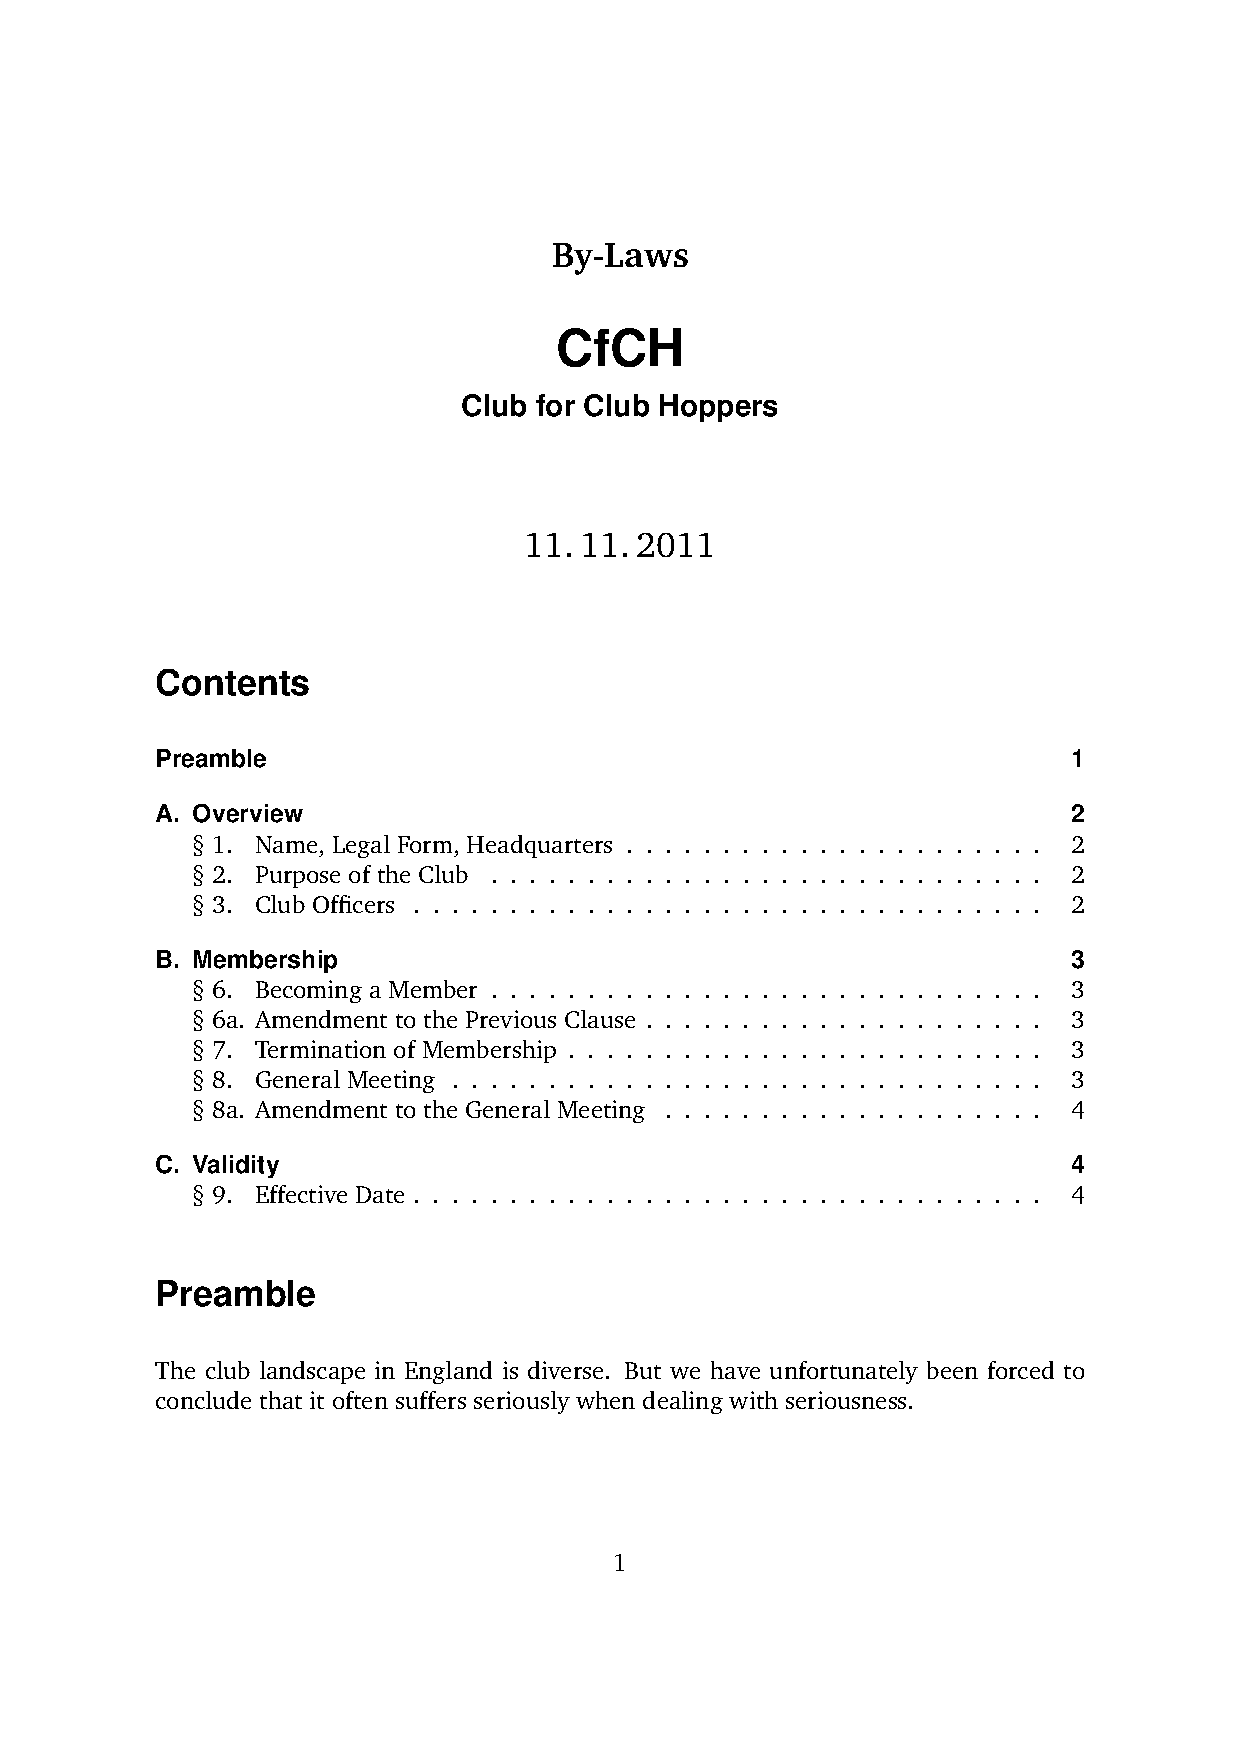
\includegraphics[page=1,width=.482\textwidth,%
        height=.49\textheight,keepaspectratio]{contract-example-en}}\enskip
      \frame{\includegraphics[page=2,width=.482\textwidth,%
        height=.49\textheight,keepaspectratio]{contract-example-en}}\par
      \smallskip}
    \begin{captionbeside}[{%
        Example: First three pages of the example club by-laws of
        \protect\autoref{sec:\LabelBase.example}%
      }]{%
        First three pages of the example club by-laws of
        \protect\autoref{sec:\LabelBase.example}%
      }%
      [l]
      \frame{\includegraphics[page=3,width=.482\textwidth,%
        height=.49\textheight,keepaspectratio]{contract-example-en}}\enskip
    \end{captionbeside}
  }{%
    {\hfill
      \frame{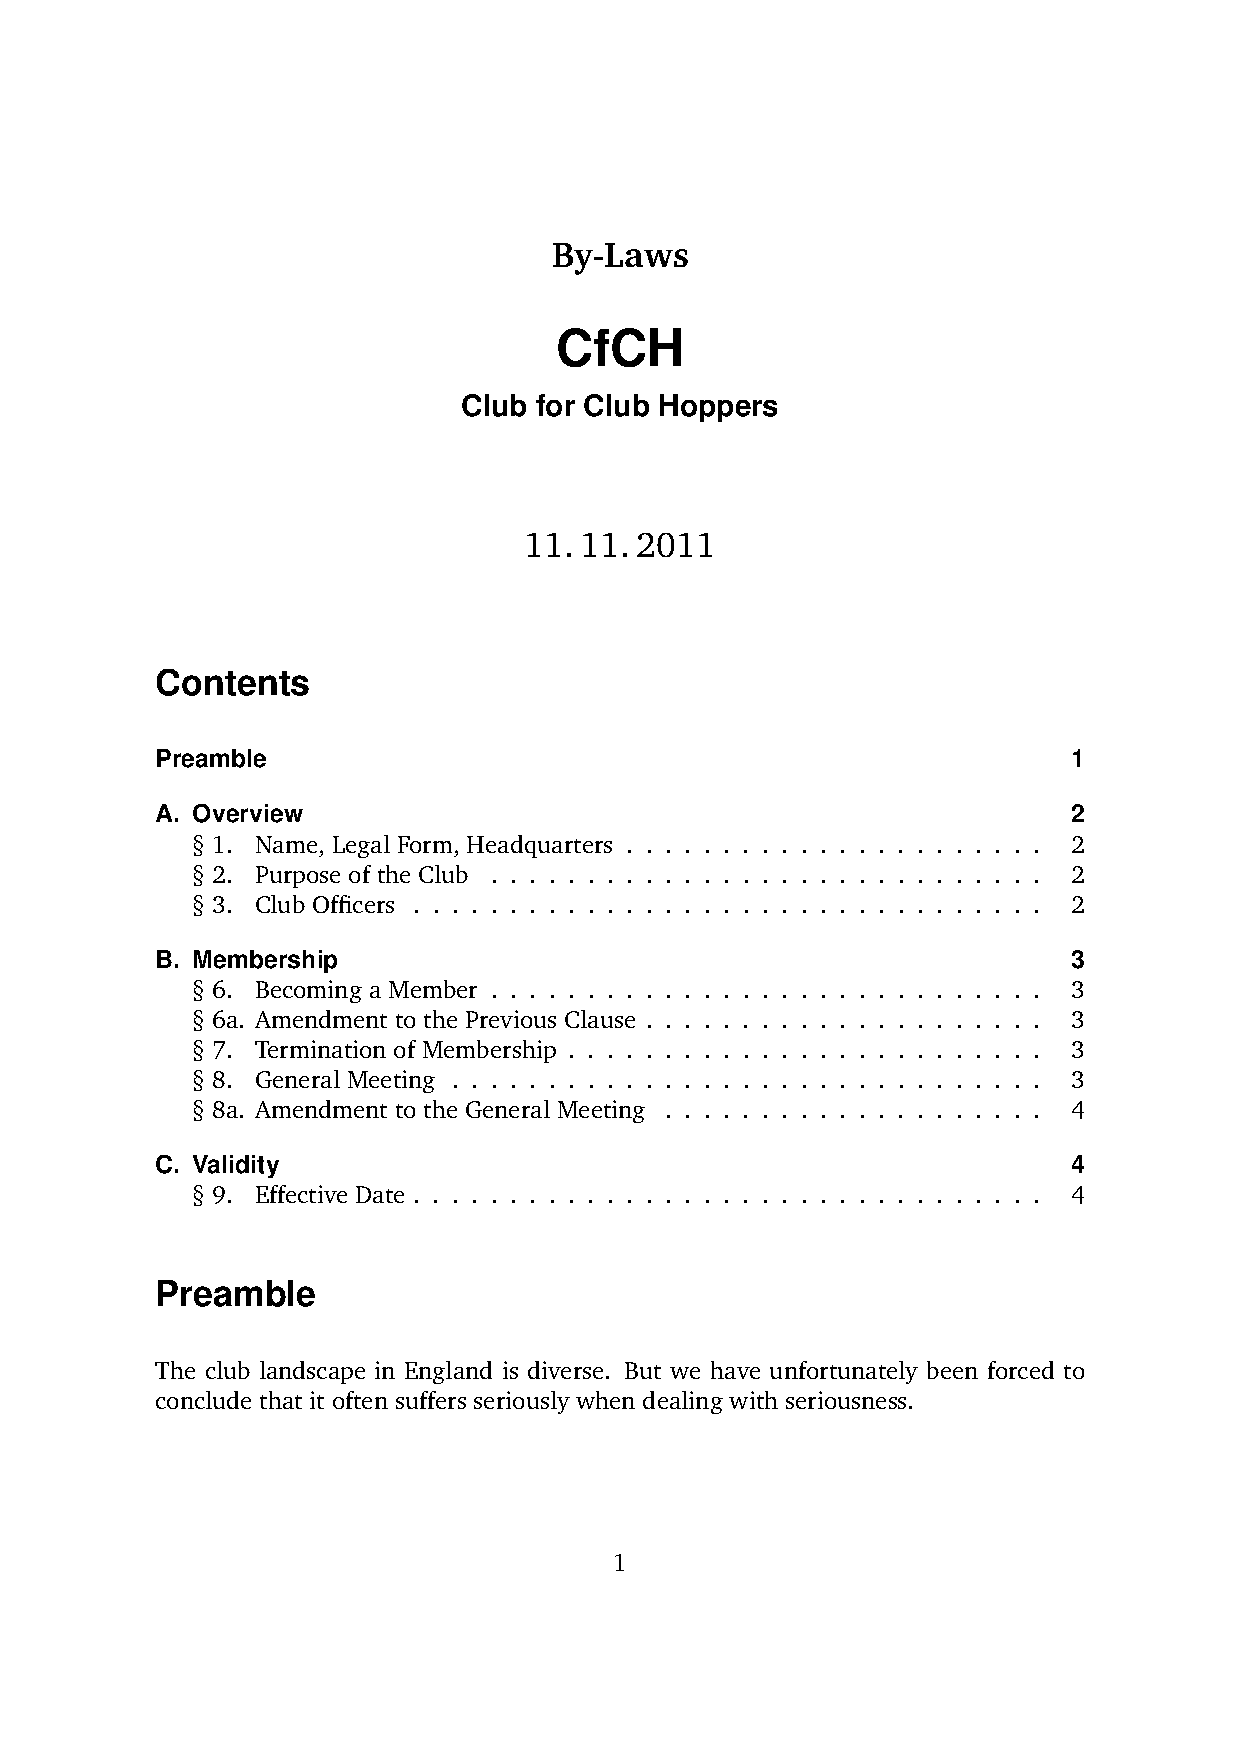
\includegraphics[page=1,width=.482\textwidth]{contract-example-en}}%
      \enskip
      \frame{\includegraphics[page=2,width=.482\textwidth]{contract-example-en}}\par
      \smallskip}
    \begin{captionbeside}[{%
        Example: First three pages of the example club by-laws of
        \protect\autoref{sec:\LabelBase.example}%
      }]{%
        First three pages of the example club by-laws of
        \protect\autoref{sec:\LabelBase.example}%
      }%
      [l]
      \frame{\includegraphics[page=3,width=.482\textwidth]{contract-example-en}}%
      \enskip
    \end{captionbeside}
  }%
  \label{fig:\LabelBase.example}
\end{figure}

\section{State of Development}
\seclabel{draft}

Since \KOMAScript~3.24, the \pkg*{contract} package has shared the version
number of the classes and other important packages of \KOMAScript.
Nevertheless, you should note that so far, the interaction of the
\DescRef{\LabelBase.env.contract} environment with the many different settings
possible with other \LaTeX{} environments, packages, or classes has not been
tested. The main reason for this is that \pkg*{contract} is very specialised
and far beyond the author's ordinary practice. So the author mostly relies on
detailed user feedback.%
\EndIndexGroup

%
%\iffalse
%</doc&en>
%<*doc&de>
%\fi
%
% \clearpage
% \selectlanguage{ngerman}
% \addpart{Benutzeranleitung}
% \renewcommand*{\LabelBase}{contract-de}
% \setcounter{section}{0}
% \renewcommand*{\thesection}{DE-\arabic{section}}
% To be added \dots
%
%\iffalse
%</doc&de>
%\fi
%
% \MaybeStop{\printbibliography[heading=bibintoc]\PrintIndex}
%
% \clearpage
% \selectlanguage{USenglish}
% \addpart{Implementation}
% \renewcommand*{\LabelBase}{contract}
% \setcounter{section}{0}
% \renewcommand*{\thesection}{\arabic{section}}
%
%    \begin{macrocode}
%<*package>
%    \end{macrocode}
%
% \changes{scrjura-v0.7b}{2014/11/11}{General renaming of ``Paragraph'' into
%   ``Clause''}
%
% \section{Cooperation with \pkg{hyperref}}
%
% If \pkg{hyperref} has already loaded before \pkg*{contract} the package cannot
% work correctly. So we throw an error. Maybe it would be a good idea to make
% this error fatal. But currently it is only an error.
%    \begin{macrocode}
%<*init>
\@ifpackageloaded{hyperref}{%
  \PackageError{contract}{Package hyperref already loaded}{%
    If you want to use package contract with package hyperref, you have
    to\MessageBreak
    load package contract before package hyperref.\MessageBreak
    To solve the problem, you just should move the loading of package
    hyperref\MessageBreak
    behind the loading of package contract.}%
}
%</init>
%    \end{macrocode}
%
% \section{Prerequisites}
%
% We need package \pkg{scrkbase}. We could load this also together with
% \pkg{tocbasic}, which is loaded later. But loading it on its own, we can
% require a minimum version.
% \begin{description}
% \item[Todo:] Package \pkg*{contract} is no longer a \KOMAScript{}
%   package. So it should not use the internal \KOMAScript{} package
%   \pkg{scrkbase}. For keys of contract environments we can just load
%   \pkg{scrbase}. For package options we should either also switch to
%   \pkg{scrbase} or use native key-value options of \LaTeX.
% \end{description}
%    \begin{macrocode}
%<*init>
\RequirePackage{scrkbase}[2013/03/26]
%</init>
%    \end{macrocode}
%
% And now, \pkg{tocbasic}.
%    \begin{macrocode}
%<*init>
\RequirePackage{tocbasic}
%</init>
%    \end{macrocode}
%
% \section{Options}
%
% \begin{option}{contract}
% \begin{macro}{\if@documentcontract,
%               \@documentcontractfalse,\@documentcontracttrue}
% \changes{scrjura-v3.36}{2022/01/25}{switched to a \KOMAScript{} option}
% Option \opt{contract} can be used to make the whole document to be a
% contract. But in this case you are not allowed to reuse the \env{contract}
% environment in the document. Nor is it allowed to stop or restart the
% contract. With older \LaTeX{} this is done by adding \cs{contract} to the
% end of \cs{document}. With an up to date \LaTeX{} we us a hook.
%    \begin{macrocode}
%<*options>
\KOMA@ifkey{contract}{@documentcontract}
\IfLTXAtLeastTF{2020/10/01}{%
  \AddToHook{begindocument/end}{%
    \RelaxFamilyKey[.contract.sty]{KOMA}{contract}%
    \if@documentcontract\expandafter\contract\fi
  }%
}{%
  \g@addto@macro\document{%
    \RelaxFamilyKey[.contract.sty]{KOMA}{contract}%
    \if@documentcontract\expandafter\contract\fi
  }%
}
%</options>
%    \end{macrocode}
% \end{macro}
% \end{option}
%
% \begin{option}{juratotoc}
% \changes{scrjura-v3.39}{2022/11/11}{initial dot in member argument of
%   option storage commands removed}
% Allow to set the toc level of the entries. Value \optvalue{true} is
% the same like \optvalue{2}, value \optvalue{false} is the same like
% \cs{maxdimen}.  \changes{scrjura-v0.7}{2013/11/04}{usage of renewed
% interface with \cs{FamilyKeyState}}
% \changes{scrjura-v0.9a}{2015/03/09}{internal value storage}
% \begin{macro}{\if@juratotoc}
% \changes{scrjura-v0.6}{2011/09/29}{replaced by counter}
% \begin{counter}{juratoclevel}
% \changes{scrjura-v0.6}{2011/09/29}{definition moved}
% \changes{scrjura-v3.27}{2019/02/25}{removed}
% \begin{macro}{\toclevel@cpar}
% \changes{scrjura-v0.7}{2013/06/09}{new, because of \pkg{hyperref}}
% \changes{scrjura-v3.27}{2019/02/25}{handled by \pkg{tocbasic}}
%    \begin{macrocode}
%<*options>
\KOMA@key{juratotoc}[true]{%
  \KOMA@set@ifkey{juratotoc}{@tempswa}{#1}%
  \ifx\FamilyKeyState\FamilyKeyStateProcessed
    \if@tempswa
      \DeclareTOCStyleEntry[level=2]{default}{cpar}%
    \else
      \DeclareTOCStyleEntry[level=\maxdimen]{default}{cpar}%
    \fi
  \else
    \DeclareTOCStyleEntry[level=#1]{default}{cpar}%
  \fi
  \KOMA@kav@xreplacevalue{contract.sty}{juratotoc}{\cpartocdepth}%
}
\KOMA@kav@xadd{contract.sty}{juratotoc}{\cpartocdepth}%
%</options>
%    \end{macrocode}
% \end{macro}
% \end{counter}
% \end{macro}
% \end{option}
%
% \begin{option}{juratocnumberwidth,juratocindent}
% \changes{scrjura-v0.6}{2011/09/29}{new}
% \changes{scrjura-v0.7}{2013/11/04}{usage of renewed interface with
%   \cs{FamilyKeyState}}
% \changes{scrjura-v0.9a}{2015/03/09}{internal value storage}
% \changes{scrjura-v3.39}{2022/11/11}{initial dot in member argument of option storage
%   commands removed}
% \begin{ilength}{\cpar@numberwidth,\cpar@indent}
% \changes{scrjura-v0.6}{2011/09/29}{new}
% \changes{scrjura-v3.27}{2019/02/25}{replaced by usage of \cs{DeclareTOCStyleEntry}}
% Indent and number width of the toc entries.
% \begin{description}
% \item[Todo:] Since we are using package \pkg{tocbasic} for the ToC entries
%   these options (and lengths) are not needed any longer, but users should
%   use \cs{DeclareTOCStyleEntry} to setup the number width and indent of the
%   entries.
% \end{description}
%    \begin{macrocode}
%<*options>
\KOMA@key{juratocnumberwidth}{%
  \DeclareTOCStyleEntry[numwidth=#1]{default}{cpar}%
  \FamilyKeyStateProcessed
  \KOMA@kav@replacevalue{contract.sty}{juratocnumberwidth}{#1}%
}
\KOMA@kav@add{contract.sty}{juratocnumberwidth}{2em}
\KOMA@key{juratocindent}{%
  \DeclareTOCStyleEntry[indent=#1]{default}{cpar}%
  \FamilyKeyStateProcessed
  \KOMA@kav@replacevalue{contract.sty}{juratocindent}{#1}%
}
\KOMA@kav@add{contract.sty}{juratocindent}{1.5em}%
%</options>
%    \end{macrocode}
% \end{ilength}
% \end{option}
%
% \begin{option}{juratitlepagebreak}
% \changes{scrjura-v0.5b}{2010/04/05}{new}
% The options sets the boolean \cs{if@juratitlepagebreak}.
% \begin{macro}{\if@juratitlepagebreak,
%               \@juratitlepagebreaktrue,\@juratitlepagebreakfalse}
% If the boolean is \cs{iftrue} page breaks inside clause headings are
% allowed (which is not recommended).
% \begin{description}
% \item[Todo:] Re-implementation either using a native key-value option (easy)
%   or a new \pkg{scrbase} family.
% \end{description}
%    \begin{macrocode}
%<*options>
\KOMA@ifkey{juratitlepagebreak}{@juratitlepagebreak}
%</options>
%    \end{macrocode}
% \end{macro}
% \end{option}
%
% \begin{option}{parnumber}
% \changes{scrjura-v0.6}{2011/09/29}{new}
% \changes{scrjura-v0.6a}{2012/10/15}{value mistake message changed}
% \changes{scrjura-v0.7}{2013/11/04}{usage of renewed interface with
%   \cs{FamilyKeyState}}
% \changes{scrjura-v0.9a}{2015/03/09}{internal value storage}
% \changes{scrjura-v3.28}{2019/11/18}{\cs{ifstr} renamed into \cs{Ifstr}}
% \changes{scrjura-v3.39}{2022/11/11}{initial dot in member argument of option storage
%   commands removed}
% The options switches the (automatic) paragraph numbering.
% \begin{description}
% \item[Todo:] Re-implementation either using a native key-value option (easy)
%   or a new \pkg{scrbase} family.
% \end{description}
%    \begin{macrocode}
%<*options>
\newif\ifparnumber
\KOMA@key{parnumber}[true]{%
  \Ifstr{#1}{auto}{%
    \AutoPar
    \FamilyKeyStateProcessed
    \KOMA@kav@remove{contract.sty}{parnumber}{manual}%
    \KOMA@kav@remove{contract.sty}{parnumber}{auto}%
    \KOMA@kav@add{contract.sty}{parnumber}{auto}%
  }{%
    \Ifstr{#1}{manual}{%
      \ManualPar
      \FamilyKeyStateProcessed
      \KOMA@kav@remove{contract.sty}{parnumber}{manual}%
      \KOMA@kav@remove{contract.sty}{parnumber}{auto}%
      \KOMA@kav@add{contract.sty}{parnumber}{manual}%
    }{%
      \KOMA@set@ifkey{parnumber}{parnumber}{#1}%
      \KOMA@kav@replacebool{contract.sty}{parnumber}{parnumber}%
    }%
  }%
}
\KOMA@kav@add{contract.sty}{parnumber}{true}
\KOMA@kav@add{contract.sty}{parnumber}{auto}
%</options>
%    \end{macrocode}
% \end{option}
%
% \begin{option}{paragraphmark,clausemark}
% \changes{scrjura-v0.9h}{2016/04/11}{\opt{paragraphmark} renamed to \opt{clausemark}}
% \changes{scrjura-v0.7}{2013/11/04}{usage of renewed interface with
%   \cs{FamilyKeyState}}
% \changes{scrjura-v0.9a}{2015/03/09}{internal value storage}
% \changes{scrjura-v3.39}{2022/11/11}{initial dot in member argument of option storage
%   commands removed}
% \begin{description}
% \item[Todo:] Re-implementation either using a native key-value option
%   or a new \pkg{scrbase} family (easy).
% \end{description}
%   \begin{option}{markright,markboth}
% \changes{scrjura-v0.7}{2013/11/04}{deprecated}
% \changes{scrjura-v3.39}{2022/11/16}{only with \KOMAScript~3}
% \begin{description}
% \item[Todo:] Remove deprecated options, because they need an internal
%   \KOMAScript{} macro.
% \end{description}
% \begin{command}{\Clausemark}
% \changes{scrjura-v0.5e}{2011/08/31}{support for \cs{MakeMarkcase}}
% The options are used to activate either \cs{markright} or \cs{markboth} for
% clauses. \cs{Clausemark} expects not only the title but also the
% number. So it differs from, e.g., \cs{chaptermark}, which uses the counter
% automatically. But maybe I will change this some time.
%    \begin{macrocode}
%<*options>
\newcommand*{\Clausemark}[1]{}
\KOMA@key{clausemark}{%
  \begingroup
    \KOMA@set@ncmdkey{clausemark}{@tempa}{%
      {false}{0},{off}{0},{no}{0},%
      {forceright}{1},%
      {forceboth}{2},%
      {right}{3},%
      {both}{4}%
    }{#1}%
  \ifx\FamilyKeyState\FamilyKeyStateProcessed
    \ifcase\number\@tempa
      \endgroup
      \let\Clausemark\@gobble
    \or
      \endgroup
      \renewcommand*{\Clausemark}[1]{%
        \markright{\csname MakeMarkcase\endcsname{##1}}}%
    \or
      \endgroup
      \renewcommand*{\Clausemark}[1]{%
        \markboth{\csname MakeMarkcase\endcsname{##1}}%
                 {\csname MakeMarkcase\endcsname{##1}}}%
    \or
      \endgroup
      \renewcommand*{\Clausemark}[1]{%
        \ifx
          \@mkboth\@gobbletwo
        \else
          \markright{\csname MakeMarkcase\endcsname{##1}}%
        \fi}%
    \or
      \endgroup
      \renewcommand*{\Clausemark}[1]{%
        \@mkboth{\csname MakeMarkcase\endcsname{##1}}%
                {\csname MakeMarkcase\endcsname{##1}}}%
    \else
      \endgroup
    \fi
    \FamilyKeyStateProcessed
  \else
    \endgroup
    \FamilyKeyStateUnknownValue
  \fi
  \KOMA@kav@xreplacevalue{contract.sty}{clausemark}{#1}%
}
\KOMA@kav@add{contract.sty}{clausemark}{false}
\@ifundefined{KOMA@DeclareDeprecatedOption}{}{%
  \KOMA@DeclareDeprecatedOption[contract]{markright}{clausemark=forceright}%
  \KOMA@DeclareDeprecatedOption[contract]{markboth}{clausemark=forceboth}%
}
\KOMA@key{paragraphmark}{%
  \PackageWarningNoLine{contract}{%
    You've used obsolete option `paragraphmark'.\MessageBreak
    Usage of this option is deprecated.\MessageBreak
    You should simply replace `paragraphmark'\MessageBreak
    by `clausemark'%
  }%
  \KOMAExecuteOptions[.contract.sty]{clausemark=#1}%
}
%</options>
%    \end{macrocode}
% \end{command}
% \end{option}
% \end{option}
%
% \begin{option}{ref}
% \changes{scrjura-v0.5d}{2010/06/07}{new values \optvalue{nopar},
%   \optvalue{nosentence}, \optvalue{OnlyParagraph}}
% \changes{scrjura-v0.7}{2013/11/04}{usage of renewed interface with
%   \cs{FamilyKeyState}}
% \changes{scrjura-v0.9a}{2015/03/09}{internal value storage}
% \changes{scrjura-v3.39}{2022/11/11}{initial dot in member argument of option
%   storage commands removed}
% \begin{description}
% \item[Todo:] Re-implementation either using a native key-value option
%   or a new \pkg{scrbase} family (easy).
% \end{description}
% \begin{option}{parcitename,sentencecitename}
% \changes{scrjura-v0.5d}{2010/06/07}{deprecated}
% \changes{scrjura-v3.39}{2022/11/16}{only with \KOMAScript~3}
% The formatting of the references of paragraphs and sentences. There are a
% long a short and a numeric form.
% \begin{description}
% \item[Todo:] Remove deprecated options, because they need an internal
%   \KOMAScript{} macro.
% \end{description}
% \begin{macro}{\parcite@format,\sentencecite@format}
% Default is the long form. Corresponding values of the two helper macros are:
% 0 = long, 1 = short, 2 = numerical, -1 = nothing.
%    \begin{macrocode}
%<*options>
\newcommand*{\parcite@format}{0}
\newcommand*{\sentencecite@format}{0}
%    \end{macrocode}
% \end{macro}
% The options can be used to change the default.
%    \begin{macrocode}
\KOMA@key{ref}{%
  \begingroup
    \KOMA@set@ncmdkey{ref}{@tempa}{%
      {parlong}{1},{longpar}{1},{ParL}{1},%
      {parshort}{2},{shortpar}{2},{ParS}{2},%
      {parnumeric}{3},{numericpar}{3},{ParN}{3},%
      {paroff}{4},{nopar}{4},%
      {sentencelong}{10},{longsentence}{10},{SentenceL}{10},%
      {sentenceshort}{20},{shortsentence}{20},{SentenceS}{20},%
      {sentencenumeric}{30},{numericsentence}{30},{SentenceN}{30},%
      {sentenceoff}{40},{nosentence}{40},%
      {long}{11},%
      {short}{22},%
      {numeric}{33},%
      {paragraphonly}{44},{onlyparagraph}{44},%
      {ParagraphOnly}{44},{OnlyParagraph}{44}%
    }{#1}%
    \ifx\FamilyKeyState\FamilyKeyStateProcessed
      \aftergroup\FamilyKeyStateProcessed
      \@tempcnta=\@tempa\relax
      \@tempcntb=\z@
      \@whilenum \@tempcnta>9 \do{%
        \advance\@tempcnta -10\relax
        \advance\@tempcntb \@ne\relax
      }%
      \ifcase \@tempcnta
      \or
        \aftergroup\def\aftergroup\parcite@format
        \aftergroup{\aftergroup0\aftergroup}%
      \or
        \aftergroup\def\aftergroup\parcite@format
        \aftergroup{\aftergroup1\aftergroup}%
      \or
        \aftergroup\def\aftergroup\parcite@format
        \aftergroup{\aftergroup2\aftergroup}%
      \or
        \aftergroup\def\aftergroup\parcite@format
        \aftergroup{\aftergroup-\aftergroup1\aftergroup}%
      \fi
      \ifcase \@tempcntb
      \or
        \aftergroup\def\aftergroup\sentencecite@format
        \aftergroup{\aftergroup0\aftergroup}%
      \or
        \aftergroup\def\aftergroup\sentencecite@format
        \aftergroup{\aftergroup1\aftergroup}%
      \or
        \aftergroup\def\aftergroup\sentencecite@format
        \aftergroup{\aftergroup2\aftergroup}%
      \or
        \aftergroup\def\aftergroup\sentencecite@format
        \aftergroup{\aftergroup-\aftergroup1\aftergroup}%
      \fi
    \else
      \aftergroup\FamilyKeyStateUnknownValue
    \fi
  \endgroup
  \ifx\FamilyKeyState\FamilyKeyStateProcessed
    \KOMA@kav@removekey{contract.sty}{ref}%
    \ifcase\parcite@format
      \KOMA@kav@add{contract.sty}{ref}{parlong}%
    \or
      \KOMA@kav@add{contract.sty}{ref}{parshort}%
    \or
      \KOMA@kav@add{contract.sty}{ref}{parnumeric}%
    \or
      \KOMA@kav@add{contract.sty}{ref}{paroff}%
    \fi
    \ifcase\sentencecite@format
      \KOMA@kav@add{contract.sty}{ref}{sentencelong}%
    \or
      \KOMA@kav@add{contract.sty}{ref}{sentenceshort}%
    \or
      \KOMA@kav@add{contract.sty}{ref}{sentencenumeric}%
    \or
      \KOMA@kav@add{contract.sty}{ref}{sentenceoff}%
    \fi
  \fi
}
\KOMA@kav@add{contract.sty}{ref}{parlong}%
\KOMA@kav@add{contract.sty}{ref}{sentencelong}%
\@ifundefined{KOMA@DeclareDeprecatedOption}{}{%
  \KOMA@DeclareDeprecatedOption[contract]{parcitename}{ref=parlong}
  \KOMA@DeclareDeprecatedOption[contract]{sentencecitename}{ref=sentencelong}
}
%</options> 
%    \end{macrocode}
% \end{option}
% \end{option}
%
% Execute the options.
%    \begin{macrocode}
%<*postoptions>
\KOMAProcessOptions\relax
%</postoptions>
%    \end{macrocode}
%
% \section{Deprecated paragraph commands}
%
% All these commands are deprecated and now generate error messages instead of
% code.
%
% \begin{command}{\Paragraph,\SubParagraph,\refParagraph,\refParagraphN,
%                 \DeprecatedParagraph,\ParagraphCompatibilityHacks}
% \changes{scrjura-v1.0}{2014/11/22}{throw error for deprecated commands but
%   only once}
% \begin{description}
% \item[Todo:] Remove deprecated commands, because they already throw errors
%   for about nine years.
% \end{description}
%    \begin{macrocode}
%<*body>
\providecommand*{\DeprecatedParagraph}{%
  \PackageError{contract}{modification of old document needed}{%
    It seem that this document was made for scrjura up to version
    0.7a.\MessageBreak
    Since scrjura version 0.9 \string\Paragraph, \string\SubParagraph, and all
    depending\MessageBreak
    commands, options, and counters have been renamed.\MessageBreak
    You should replace the terms `Paragraph' and `paragraph` by `Clause`
    and\MessageBreak
    `clause` if they are part of the name of a contract feature, otherwise
    this\MessageBreak
    document may produce severall additional error messages and maybe the
    wrong\MessageBreak
    result. Sorry for the inconvenience.%
  }%
  \ParagraphCompatibilityHacks
}
\newcommand*{\ParagraphCompatibilityHacks}{%
  \PackageWarning{contract}{compatibility hacks for `\string\Paragraph'
    executed.\MessageBreak
    There is no support for documents using these hacks!\MessageBreak
    There is no warranty for real compatibility!\MessageBreak
    Even if the LaTeX run of the document doesn't report\MessageBreak
    any error, the result may be completely wrong.\MessageBreak
    Therefore it is recommended to solve the problem,\MessageBreak
    instead of trying to work around using the\MessageBreak
    compatibility hacks%
  }%
  \gdef\Paragraph{\Clause}%
  \gdef\SubParagraph{\SubClause}%
  \gdef\c@Paragraph{\c@Clause}%
  \gdef\cl@Paragraph{\cl@Clause}%
  \gdef\c@SubParagraph{\c@SubClause}%
  \gdef\cl@SubParagraph{\cl@SubClause}%
  \gdef\theParagraph{\theClause}%
  \gdef\theSubParagraph{\theSubClause}%
  \gdef\refParagraph{\refClause}%
  \gdef\refParagraphN{\refClauseN}%
  \aliaskomafont{Paragraph}{Clause}%
  \scr@ifundefinedorrelax{Paragraphmark}{}{%
    \global\let\Clausemark\Paragraphmark
  }%
}
\providecommand*{\Paragraph}{\DeprecatedParagraph\Paragraph}
\providecommand*{\SubParagraph}{\DeprecatedParagraph\SubParagraph}
\providecommand*{\refParagraph}{\DeprecatedParagraph\refParagraph}
\providecommand*{\refParagraphN}{\DeprecatedParagraph\refParagraphN}
%</body>
%    \end{macrocode}
% \end{command}
%
%
% \section{Contracts, clauses, paragraphs and sentences}
%
%
% \begin{macro}{\contract@env@type}
% \changes{scrjura-v0.5d}{2010/04/28}{new}
% \changes{scrjura-v0.7b}{2014/11/03}{\cs{jura@env@type} renamed}
% \changes{v0.0.1}{2023-10-10}{\cs{scrjura@env@type} renamed}
% This macro shows the currently active \pkg*{contract} environment.
%    \begin{macrocode}
%<*body>
\newcommand*{\contract@env@type}{}
%</body>
%    \end{macrocode}
% \end{macro}
%
%
% \begin{command}{\ellipsispar}
% \changes{scrjura-v0.7}{2013/05/02}{new}
% \changes{scrjura-v0.7b}{2014/11/03}{\cs{thecontractAbsoluteClause} made more
%   flexible}
% \changes{scrjura-v0.9g}{2016/03/25}{write to \file{aux}-file only \cs{if@filesw}}
% \begin{command}{\parellipsis}
% \changes{scrjura-v0.7}{2013/05/02}{new}
% Count one or more paragraphs given by the optional argument but print
% \cs{parellipsis} instead of a real paragraph. The default is either
% \cs{dots} or \cs{textellipsis} if available.
% \changes{scrjura-v0.7}{2013/05/02}{new}
%    \begin{macrocode}
%<*body>
\newcommand*{\ellipsispar}[1][1]{%
  \begingroup
    \KOMAoptions{parnumber=manual}\parellipsis\par
    \addtocounter{par}{#1}%
    \if@filesw
      \protected@write\@auxout{}{%
        \string\newmaxpar{\contract@env@type}%
                         {\csname the\contract@env@type 
                           AbsoluteClause\endcsname}%
                         {\thepar}%
      }%
    \fi
  \endgroup
  \addtocounter{par}{-1}\refstepcounter{par}%
  \ignorespaces
}
\newcommand*{\parellipsis}{%
  \scr@ifundefinedorrelax{textellipsis}{\dots}{\textellipsis}%
}
%</body>
%    \end{macrocode}
% \end{command}
% \end{command}
%
% \begin{environment}{contract}
% \changes{scrjura-v0.5d}{2010/04/28}{missing error message added}
% \changes{scrjura-v0.5d}{2010/04/28}{not self-redefining any more}
% \changes{scrjura-v0.5d}{2010/04/28}{defining \cs{jura@env@type}}
% \changes{scrjura-v3.36}{2022/01/25}{defining an environment (because of hooks)}
% \begin{macro}{\if@contract@skiphyperref}
% \changes{v0.0.1}{2023-10-10}{\cs{if@scrjura@skiphyperref} renamed}
% \begin{counter}{contractClause}
% \begin{command}{\thecontractClause}
% \changes{scrjura-v0.9b}{2015/05/01}{must use counter \cnt{Clause} instead of
%   \cnt{contractClause}}
% \begin{macro}{\contract@Clauseformat}
% \begin{command}{\Clauseformat,\paragraphformat}
% \changes{scrjura-v0.6b}{2013/04/16}{redefinition of \cs{paragraphformat}}
% \begin{counter}{contractSubClause}
% \changes{scrjura-v0.9b}{2015/05/01}{must use counter \cnt{SubClause} instead of
%   \cnt{contractSubClause}}
% \begin{command}{\thecontractSubClause}
% \begin{counter}{contractAbsoluteClause}
% \changes{scrjura-v0.7}{2013/04/18}{new (internal) counter for all clauses to make
%   it possible to reset the users clause counter}
% It is not allowed to nest the \env{contract} environments, but you can end
% them and start them new. But this would not end the contract and start a new
% contract but only delay it for some other code.
%    \begin{macrocode}
%<*body>
\newenvironment{contract}{%
  \ifx\contract@env@type\@empty
    \let\@doendpe\contract@doendpe
    \let\Clause\contract@paragraph
    \let\c@Clause\c@contractClause
    \edef\cl@Clause{\cl@Clause\cl@contractClause}%
    \let\SubClause\contract@subparagraph
    \let\c@SubClause\c@contractSubClause
    \edef\cl@SubClause{\cl@SubClause\cl@contractSubClause}%
    \let\Sentence\contract@sentence
    \renewcommand*{\contract@env@type}{contract}%
    \aliaskomafont{Clause}{contract.Clause}%
  \else
    \PackageError{contract}{nested `contract` detected}{%
      You may not use a `contract' environment inside\MessageBreak
      a `\contract@env@type' environment or after loading\MessageBreak
      package `contract' with option `\contract@env@type'!}%
  \fi
}{}
\let\if@contract@skiphyperref\iftrue
\let\cl@Clause\@empty
\let\cl@SubClause\@empty
\newcounter{contractClause}
\renewcommand*{\thecontractClause}{%
  {\contract@Clauseformat{\arabic{Clause}}}}
\DeclareRobustCommand*{\contract@Clauseformat}[1]{\Clauseformat{#1}}
\newcommand*{\Clauseformat}[1]{\S~#1}
\newcounter{contractSubClause}
\@addtoreset{SubClause}{Clause}
\renewcommand*{\thecontractSubClause}{%
  {\theClause\alph{SubClause}}}
\newcounter{contractAbsoluteClause}
%</body>
%    \end{macrocode}
% \end{counter}
% \end{command}
% \end{counter}
% \end{command}
% \end{macro}
% \end{command}
% \end{counter}
% \end{macro}
% \end{environment}
%
% \begin{command}{\DeclareNewJuraEnvironment}
% \changes{scrjura-v0.9}{2014/11/12}{new}
% \changes{scrjura-v0.9h}{2016/04/12}{\cs{@ifnextchar} replaced by
%   \cs{kernel@ifnextchar}}
% Using \cs{@defjuraenvironment} to define a new juristic environment. This
% can be done only in document preamble.
%    \begin{macrocode}
%<*body>
\newcommand*{\DeclareNewJuraEnvironment}[1]{%
  \@ifundefined{#1}{\expandafter\let\csname #1\expandafter\endcsname
    \csname end#1\endcsname}{}%
  \@ifundefined{#1}{\let\reserved@defjuraenvironment\@defjuraenvironment}{%
    \PackageError{contract}{ignorring declaration of `#1'}{%
      You've tried to declare jura environment `#1', but
      environment\MessageBreak
      `#1' or command
      \expandafter\string\csname #1\endcsname\space or
      \expandafter\string\csname end#1\endcsname\MessageBreak
      already exists.\MessageBreak
      Declaration will be ignored}%
    \long\def\reserved@defjuraenvironment##1[##2]##3##4{}%
  }%
  \kernel@ifnextchar [%]
    {\reserved@defjuraenvironment{#1}}{\reserved@defjuraenvironment{#1}[]}%
}
\@onlypreamble\DeclareNewJuraEnvironment
%    \end{macrocode}
% \begin{macro}{\@defjuraenvironment}
% \changes{scrjura-v0.9}{2014/11/04}{new}
% \changes{scrjura-v3.25}{2017/12/08}{new command options \opt{ClauseFont}}
% \changes{scrjura-v3.25}{2017/12/08}{\cs{reserved@defjuraenvironment} set back to
%   \cs{relax}}
% \changes{scrjura-v3.25}{2017/12/08}{using local instead of global command options}
% This command is used to define a new \pkg*{contract} environment like
% \env{contract}. Several options are provided (see the user manual for
% details).
%    \begin{macrocode}
\DefineFamily{KOMAarg}
\DefineFamilyMember{KOMAarg}
\newcommand{\@defjuraenvironment}{}
\long\def\@defjuraenvironment#1[#2]#3#4{%
  \let\reserved@defjuraenvironment\relax
%    \end{macrocode}
% The counters:
%    \begin{macrocode}
  \newcounter{#1Clause}%
  \newcounter{#1AbsoluteClause}%
  \newcounter{#1SubClause}%
  \FamilyCSKey[.contract.sty]{KOMAarg}{Clause}{#1@Clause}%
  \FamilyCSKey[.contract.sty]{KOMAarg}{SubClause}{#1@SubClause}%
  \FamilyCSKey[.contract.sty]{KOMAarg}{Sentence}{#1@Sentence}%
  \DefineFamilyKey[.contract.sty]{KOMAarg}{ClauseNumberFormat}{%
    \expandafter\def\csname #1@Clauseformat \endcsname####1{##1{####1}}%
    \expandafter\edef\csname #1@Clauseformat\endcsname{%
      \noexpand\protect\expandafter\noexpand\csname #1@Clauseformat \endcsname
    }%
    \FamilyKeyStateProcessed
  }
  \DefineFamilyKey[.contract.sty]{KOMAarg}{ClauseFont}{%
    \IfExistskomafont{#1.Clause}{%
      \IfIsAliaskomafont{#1.Clause}{%
        \expandafter\let\csname scr@fnt@instead@#1.Clause\endcsname\relax
        \newkomafont{#1.Clause}{##1}%
      }{\setkomafont{#1.Clause}{##1}}%
    }{%
      \newkomafont{#1.Clause}{##1}%
    }%
  }
  \FamilyExecuteOptions[.contract.sty]{KOMAarg}{#2}%
  \RelaxFamilyKey[.contract.sty]{KOMAarg}{ClauseFont}%
  \RelaxFamilyKey[.contract.sty]{KOMAarg}{ClauseNumberFormat}%
  \RelaxFamilyKey[.contract.sty]{KOMAarg}{Sentence}%
  \RelaxFamilyKey[.contract.sty]{KOMAarg}{SubClause}%
  \RelaxFamilyKey[.contract.sty]{KOMAarg}{Clause}%
  \@ifundefined{#1@Clauseformat}{%
    \expandafter\DeclareRobustCommand\expandafter*%
    \csname #1@Clauseformat\endcsname[1]{\Clauseformat{##1}}%
  }{}%
%    \end{macrocode}
% \changes{scrjura-v0.9c}{2015/05/13}{defining \cs{the\dots Clause}}
% \changes{scrjura-v0.9f}{2016/02/24}{\cs{protect}\cs{@nameuse} instead of
%     \cs{csname}\dots\cs{endcsname}}
%    \begin{macrocode}
  \expandafter\renewcommand\expandafter*\csname the#1Clause\endcsname{%
    \protect\@nameuse{#1@Clauseformat}{\arabic{#1Clause}}}%
%    \end{macrocode}
% Environment:
%    \begin{macrocode}
  \newenvironment{#1}{%
    \par
    \ifx\contract@env@type\@empty
      \edef\contract@env@type{#1}%
      \let\@doendpe\contract@doendpe
      \expandafter\let\expandafter\c@Clause\csname c@#1Clause\endcsname
      \edef\cl@Clause{\cl@Clause\csname cl@#1Clause\endcsname}%
      \expandafter\let\expandafter\c@SubClause
        \csname c@#1SubClause\endcsname
      \edef\cl@SubClause{\cl@SubClause
        \csname cl@#1SubClause\endcsname}%
      \@ifundefined{#1@Clause}{%
        \let\Clause\contract@paragraph
      }{%
        \expandafter\let\expandafter\Clause
        \csname #1@Clause\endcsname
      }%
      \@ifundefined{#1@SubClause}{%
        \let\SubClause\contract@subparagraph
      }{%
        \expandafter\let\expandafter\SubClause
        \csname #1@SubClause\endcsname
      }%
      \@ifundefined{#1@Sentence}{%
        \let\Sentence\contract@sentence
      }{%
        \expandafter\let\expandafter\Sentence\csname #1@Sentence\endcsname
      }%
      \@ifundefined{\contract@env@type @everypar}{%
        \expandafter\let
        \csname \contract@env@type @everypar\endcsname
        \contract@everypar
      }{}%
%    \end{macrocode}
% Font alias for \fnt{Clause}. If neither a font not an alias is defined for
% the new environment \fnt{contract.Clause} is used.
% \changes{scrjura-v3.25}{2017/12/08}{Font alias fixed}
%    \begin{macrocode}
      \IfExistskomafont{#1.Clause}{%
        \IfIsAliaskomafont{#1.Clause}{%
          \aliaskomafont{Clause}{\csname scr@fnt@instead@#1.Clause\endcsname}%
        }{%
          \aliaskomafont{Clause}{#1.Clause}%
        }%
      }{%
        \aliaskomafont{Clause}{contract.Clause}%
      }%
      #3%
    \else
      \PackageError{contract}{nested contract environments detected}{%
        You must not use a `#1' environment inside\MessageBreak
        a `\contract@env@type' environment or after loading\MessageBreak
        package `contract' with option `\contract@env@type'!}%
    \fi
  }{%
    #4%
    \par
  }%
}
%</body>
%    \end{macrocode}
% \end{macro}%^^A \@dewjuraenvironment
% \end{command}%^^A \DeclareNewJuraEnvironment
%
% \begin{macro}{\contract@paragraph}
% This is the \cs{Clause} used by contracts. A contract consists (usually) of
% several clauses. Each clause has optional elements managed by
% \meta{key}=\meta{value} pairs handled by \pkg{scrkbase} and last but not
% least by \pkg{keyval}.
% \begin{option}{title,head,nohead}
% \begin{option}{entry,noentry}
% \changes{scrjura-v0.6}{2011/09/30}{deprecated}
% \begin{option}{tocentry,notocentry}
% \changes{scrjura-v0.6}{2011/09/30}{new}
% Title, running head and toc entry of the clause. The title is the default
% for running head and toc entry. But you can also use an empty value for
% each of them or use the \opt{no\dots} options to switch them off.
%    \begin{macrocode}
%<*body>
\define@key{contract}{title}{%
  \def\contract@title{#1}%
  \ifx\contract@entry\relax\def\contract@entry{\contract@title}\fi
  \ifx\contract@head\relax\def\contract@head{\contract@title}\fi
}
\define@key{contract}{entry}{%
  \PackageWarning{contract}{deprecated option `entry'.\MessageBreak
    You should use option `tocentry' instead of\MessageBreak
    option `entry'%
  }%
  \def\contract@entry{#1}}
\define@key{contract}{tocentry}{\def\contract@entry{#1}}
\define@key{contract}{noentry}[]{%
  \PackageWarning{contract}{deprecated option `noentry'.\MessageBreak
    You should use option `notocentry' instead of\MessageBreak
    option `noentry'%
  }%
  \let\contract@entry\relax}
\define@key{contract}{notocentry}[]{\let\contract@entry\relax}
\define@key{contract}{head}{\def\contract@head{#1}}
\define@key{contract}{nohead}[]{\let\contract@head\relax}
%    \end{macrocode}
% \end{option}
% \end{option}
% \end{option}
% \begin{option}{number}
% The number can be changed manually. But clauses without numbers are not
% allowed. So if you use an empty value, the number is automatically set.
%    \begin{macrocode}
\define@key{contract}{number}{\def\contract@number{#1}}
%    \end{macrocode}
% \end{option}
% \begin{macro}{\contract@preskip,\contract@postskip}
% \begin{option}{preskip,postskip}
% The options are used to specify the distance before and after the
% clause. The preset value of these options are the global settings done by
% |\setkeys{contract}{…}|.
%    \begin{macrocode}
\newcommand*{\contract@preskip}{2\baselineskip}
\newcommand*{\contract@postskip}{\baselineskip}
\define@key{contract}{preskip}{\def\contract@preskip{#1}}
\define@key{contract}{postskip}{\def\contract@postskip{#1}}
%    \end{macrocode}
% \end{option}
% \end{macro}
% \begin{option}{dummy}
% The option switches the boolean \cs{ifcontract@dummy}.
% \begin{macro}{\ifcontract@dummy}
% If the boolean is \cs{iftrue} the clause will not be printed. But note: you
% cannot use this to remove the paragraphs or sentences of the clause. But you
% can use this option to generate holes in the numbering without manually
% manipulating the counters.
%    \begin{macrocode}
\newif\ifcontract@dummy
\define@key{contract}{dummy}[true]{\csname contract@dummy#1\endcsname}
%    \end{macrocode}
% \end{macro}
% \end{option}
% \begin{fontelement}{contract.Clause}
% \begin{macro}{\contract@paragraph@font}
% \changes{scrjura-v3.25}{2017/12/08}{using element \fnt{Clause} instead of
%   \fnt{contract.Clause}}
% Correctly this macro should be named \cs{contract@paragraph@format}. But it
% is already used by some users for ugly tricks. So I will not rename it to
% avoid problems for existing documents. Additionally it would be better to
% use a new macro per environment. However the same reason not to change this.
%    \begin{macrocode}
\newkomafont{contract.Clause}{\sffamily\bfseries\large}
\newcommand*{\contract@paragraph@font}{\usekomafont{Clause}%
  \@hangfrom}
%    \end{macrocode}
% \end{macro}
% \end{fontelement}
% \begin{counter}{@AbsClause}
% \begin{macro}{\theH@AbsClause}
% \changes{scrjura-v3.41}{2023/06/24}{Ulrike Fischer requested to use \cs{def} instead
%   of \cs{newcommand*}}
% \begin{command}{\theHClause,\theHSubClause}
% \changes{scrjura-v3.41}{2023/06/24}{Ulrike Fischer requested to use \cs{def} instead
%   of \cs{newcommand*}}
%    \begin{macrocode}
% Here we have some not good tested code for \pkg{hyperref}.
\newcounter{@AbsClause}
\def\theH@AbsClause{P-\arabic{@AbsClause}}
\def\theHClause{\theH@AbsClause}
\def\theHSubClause{\theH@AbsClause}
%    \end{macrocode}
% \end{command}
% \end{macro}
% \end{counter}
% For the headings we use manual paragraph numbering, because we don't want
% any paragraph numbering inside the heading. After initializing the options
% they are processed.
% \changes{scrjura-v0.7}{2013/04/18}{increase counter \cnt{contractAbsoluteClause}}
% \changes{scrjura-v0.7b}{2014/11/03}{more flexible
%   \cnt{\meta{environment}AbsoluteClause}}
%    \begin{macrocode}
\newcommand*{\contract@paragraph}[1]{%
  \stepcounter{\contract@env@type AbsoluteClause}%
  \ManualPar\parnumbertrue
  \let\contract@title\relax
  \let\contract@entry\relax
  \let\contract@head\relax
  \let\contract@number\relax
  \contract@dummyfalse
  \ifx\relax#1\relax\else\setkeys{contract}{#1}\fi
%    \end{macrocode}
% Unless this is a dummy clause, the headings will be initialized and vertical
% skips will be done.
% \changes{scrjura-v0.6a}{2012/10/08}{missing \cs{par} added}
%    \begin{macrocode}
  \ifcontract@dummy\else
    \par
    \@afterindentfalse
    \addvspace{\contract@preskip}%
  \fi
%    \end{macrocode}
% If there isn't a manual number, we use the next number. If there is a manual
% number, this number is printed and we take care that labels and
% \pkg{hyperref} also use the manual number.
% \changes{scrjura-v0.6b}{2013/04/16}{using \cs{contract@Clauseformat} for manual
%   numbers too}
% \changes{scrjura-v0.9c}{2015/05/13}{\cs{thecontractClause} replaced by
%   environment-dependent macro}
%    \begin{macrocode}
  \ifx\contract@number\relax
    \let\p@Clause\@empty
    \expandafter\let\expandafter\theClause
      \csname the\contract@env@type Clause\endcsname
    \refstepcounter{Clause}%
  \else
    \begingroup
      \let\@elt\@stpelt
      \cl@Clause
    \endgroup
%    \end{macrocode}
% \changes{scrjura-v0.9f}{2016/02/24}{\cs{protect}\cs{@nameuse} instead of
%   \cs{csname}\dots\cs{endcsname}}
% \changes{scrjura-v3.41}{2023/06/24}{update of \cs{@currentcounter} added}
%    \begin{macrocode}
    \protected@edef\theClause{%
      \protect\@nameuse{\contract@env@type @Clauseformat}{\contract@number}%
    }%
    \protected@edef\@currentlabel{\theClause}%
    \def\@currentcounter{Clause}%
  \fi
  \stepcounter{@AbsClause}%
  \begingroup\expandafter\expandafter\expandafter\endgroup
  \expandafter\ifx\csname if@skiphyperref\endcsname\relax
  \else
    \expandafter\let\csname if@contract@skiphyperref\expandafter\endcsname
    \csname if@skiphyperref\endcsname
  \fi
  \if@contract@skiphyperref\else
    \hyper@refstepcounter{@AbsClause}%
    \typeout{absolute Nummer: \the@AbsClause^^JLabel: `\@currentHref'}%
  \fi
%    \end{macrocode}
% For simplification we use the code of clauses for sub-clauses.
%    \begin{macrocode}
  \let\theSubClause\theClause
%    \end{macrocode}
% Unless for dummy clauses, the heading is printed, the toc entry is done
% and also the running head.
% \changes{scrjura-v0.7}{2013/04/28}{distance behind the number is part of the number}
% \changes{scrjura-v0.9i}{2017/02/23}{usage of \cs{ext@toc}}
%    \begin{macrocode}
  \ifcontract@dummy\else
    \begingroup
      \if@juratitlepagebreak\else\interlinepenalty\@M\fi
      \contract@paragraph@font{\theClause
        \ifx\contract@title\relax\else\enskip\fi}%
      \contract@title
      \ifx\contract@entry\relax\else
        \expandafter\addxcontentsline\expandafter{\ext@toc}%
        {cpar}[\theClause]\contract@entry
        \addxcontentsline{cpa}{cpar}[\theClause]\contract@entry
      \fi
      \ifx\contract@head\relax\else
        \expandafter\Clausemark\expandafter{%
          \expandafter\theSubClause\expandafter\enskip\contract@head}%
      \fi
      \par
    \endgroup\nobreak\vskip\contract@postskip
%    \end{macrocode}
% Last but not least paragraph numbering is initialized.
%    \begin{macrocode}
    \contract@afterheading
  \fi
}
%</body>
%    \end{macrocode}
% \end{macro}
%
% \begin{macro}{\contract@subparagraph}
% \changes{scrjura-v0.6a}{2012/10/08}{fehlendes \cs{par} ergänzt}
% \changes{scrjura-v0.7}{2013/04/18}{Zähler \texttt{contractAbsoluteClause} wird
%   erhöht}
% \changes{scrjura-v0.7}{2013/04/28}{Abstand nach der Nummer als Bestandteil der
%   Nummer setzen}
% \changes{scrjura-v0.9i}{2017/02/23}{Verwendung von \cs{ext@toc}}
% \changes{scrjura-v3.41}{2023/06/24}{update of \cs{@currentcounter} added}
% Das entspricht bis auf wenige Kleinigkeiten, die Unterparagraphen betreffen,
% |\contract@paragraph|
%    \begin{macrocode}
%<*body>
\newcommand*{\contract@subparagraph}[1]{%
  \stepcounter{\contract@env@type AbsoluteClause}%
  \ManualPar\parnumbertrue
  \let\contract@title\relax
  \let\contract@entry\relax
  \let\contract@head\relax
  \let\contract@number\relax
  \contract@dummyfalse
  \ifx\relax#1\relax\else\setkeys{contract}{#1}\fi
  \ifcontract@dummy\else
    \par
    \@afterindentfalse
    \vskip\contract@preskip
  \fi
  \ifx\contract@number\relax
    \let\p@SubClause\@empty
    \let\theSubClause\thecontractSubClause
    \refstepcounter{SubClause}%
  \else
    \begingroup
      \let\@elt\@stpelt
      \cl@SubClause
    \endgroup
    \protected@edef\theSubClause{\theClause\contract@number}%
    \protected@edef\@currentlabel{\theSubClause}%
    \def\@currentcounter{SubClause}%
  \fi
  \stepcounter{@AbsClause}%
  \begingroup\expandafter\expandafter\expandafter\endgroup
  \expandafter\ifx\csname if@skiphyperref\endcsname\relax
  \else
    \expandafter\let\csname if@contract@skiphyperref\expandafter\endcsname
    \csname if@skiphyperref\endcsname
  \fi
  \if@contract@skiphyperref\else
    \hyper@refstepcounter{@AbsClause}%
    \typeout{absolute Nummer: \the@AbsClause^^JLabel: `\@currentHref'}%
  \fi
  \ifcontract@dummy\else
    \begingroup
      \if@juratitlepagebreak\else\interlinepenalty\@M\fi
      \contract@paragraph@font{\theSubClause
        \ifx\contract@title\relax\else\enskip\fi}%
      \contract@title
      \ifx\contract@entry\relax\else
        \expandafter\addxcontentsline\expandafter{\ext@toc}%
        {cpar}[\theSubClause]\contract@entry
        \addxcontentsline{cpa}{cpar}[\theSubClause]\contract@entry
      \fi
      \ifx\contract@head\relax\else
        \expandafter\Clausemark\expandafter{%
          \expandafter\theSubClause\expandafter\enskip\contract@head}%
      \fi
      \par
    \endgroup
    \nobreak\vskip\contract@postskip
    \contract@afterheading
  \fi
}
%</body>
%    \end{macrocode}
% \end{macro}
%
% \begin{command}{\AutoPar,\ManualPar}
% Switching between automatic or manual paragraph numbers for all
% \pkg*{contract} environments.
%    \begin{macrocode}
%<*body>
\newcommand*{\AutoPar}{%
  \expandafter\let\expandafter\contract@used@everypar
  \csname \contract@env@type @everypar\endcsname
}
\newcommand*{\ManualPar}{%
  \let\contract@used@everypar\relax
}
%</body>
%    \end{macrocode}
% \end{command}
%
% \begin{macro}{\contract@afterheading}
% \changes{scrjura-v0.7b}{2014/11/03}{\cs{jura@afterheading} renamed}
% \changes{scrjura-v0.7b}{2014/11/03}{no argument}
% \changes{scrjura-v3.27}{2019/02/25}{\cs{CheckCommand} for \cs{@afterheading}}
% \changes{v0.0.1}{2023-10-10}{\cs{scrjura@afterheading} renamed}
% Similar to \cs{afterheading} but with automatic paragraph numbers.
% \begin{description}
% \item[ToDo:] Test if this can be done using \LaTeX{} hooks, depending on the
%   \LaTeX{} release.
% \end{description}
%    \begin{macrocode}
%<*body>
\CheckCommand*{\@afterheading}{%
  \@nobreaktrue
  \everypar{%
    \if@nobreak
      \@nobreakfalse
      \clubpenalty \@M
      \if@afterindent \else
        {\setbox\z@\lastbox}%
      \fi
    \else
      \clubpenalty \@clubpenalty
      \everypar{}%
    \fi}%
}
\newcommand*{\contract@afterheading}{%
  \@nobreaktrue
  \everypar{%
    \if@nobreak
      \@nobreakfalse
      \clubpenalty \@M
      \if@afterindent \else
        {\setbox\z@\lastbox}%
      \fi
    \else
      \clubpenalty \@clubpenalty
      \everypar{%
        \contract@used@everypar
      }%
    \fi
    \contract@used@everypar
  }%
  \AutoPar
}
%    \end{macrocode}
% \begin{macro}{\contract@used@everypar}
% \changes{scrjura-v0.7b}{2014/11/03}{\cs{jura@everypar} renamed}
% \changes{v0.0.1}{2023-10-10}{\cs{scrjura@everypar} renamed}
% The macro to be used at the very beginning of every paragraph to add the
% number. To be used only inside \pkg*{contract} environments, so empty
% outside.
%    \begin{macrocode}
\newcommand*{\contract@used@everypar}{}
%    \end{macrocode}
% \end{macro}
% \begin{macro}{\@doendpe}
% \LaTeX{} used this macro, to reset all paragraph actions at the end of
% environments. To avoid unwanted switching-off of the paragraph number it
% will be reinitialized.
% \begin{macro}{\contract@doendpe}
% \changes{v0.0.1}{2023-10-10}{\cs{scrjura@doendpe} renamed}
% \begin{macro}{\IncludeInRelease}
% \changes{scrjura-v0.9e}{2015/11/03}{used temporary}
% \changes{scrjura-v3.28}{2019/11/18}{\cs{ifstr} renamed into \cs{Ifstr}}
% \begin{macro}{\@gobble@IncludeInRelease}
% \changes{scrjura-v0.9e}{2015/11/03}{used temporary}
% \begin{macro}{\EndIncludeInRelease}
% \changes{scrjura-v0.9e}{2015/11/03}{used temporary}
% From \LaTeX{} 2015/01/01 a different definition of \cs{@doendpe} is used. So
% we also have to use different versions depending on the release. We do so
% with some tricks. Maybe this should be replaced by usage of
% \cs{IfLTXAtLeastTF} from already loaded \pkg{scrbase}.
% \begin{description}
% \item[Todo:] Using \cs{everypar} is evil and should be replaced by using a
%   generic paragraph hook.
% \end{description}
%    \begin{macrocode}
\providecommand*{\IncludeInRelease}[3]{%
  \PackageInfo{contract}{temporary definition of \string\IncludeInRelease}%
  \Ifstr{#1}{0000/00/00}{%
    \let\IncludeInRelease\@undefined
    \def\EndIncludeInRelease{\let\EndIncludeInRelease\@undefined}%
  }{%
    \let\EndIncludeInRelease\relax
    \long\def\@gobble@IncludeInRelease##1\EndIncludeInRelease{%
      \let\@gobble@IncludeInRelease\@undefined
    }%
    \expandafter\@gobble@IncludeInRelease
  }%
}
\IncludeInRelease{2015/01/01}{\@doendpe}{clubpenalty fix}
\CheckCommand*\@doendpe{\@endpetrue
     \def\par{\@restorepar
              \clubpenalty\@clubpenalty
              \everypar{}\par\@endpefalse}\everypar
               {{\setbox\z@\lastbox}%
                \everypar{}\@endpefalse}}
\newcommand*{\contract@doendpe}{%
  \@endpetrue
  \def\par{%
    \@restorepar
    \clubpenalty\@clubpenalty
    \everypar{%
      \csname contract@used@everypar\endcsname
    }%
    \par\@endpefalse
  }%
  \everypar{%
    {\setbox\z@\lastbox}\everypar{%
      \csname contract@used@everypar\endcsname
    }%
    \@endpefalse
  }%
}
\EndIncludeInRelease
\IncludeInRelease{0000/00/00}{\@doendpe}{clubpenalty fix}
\CheckCommand*\@doendpe{\@endpetrue
  \def\par{\@restorepar\everypar{}\par\@endpefalse}\everypar
  {{\setbox\z@\lastbox}\everypar{}\@endpefalse}}
\newcommand*{\contract@doendpe}{%
  \@endpetrue
  \def\par{%
    \@restorepar\everypar{%
      \csname contract@used@everypar\endcsname
    }%
    \par\@endpefalse
  }%
  \everypar{%
    {\setbox\z@\lastbox}\everypar{%
      \csname contract@used@everypar\endcsname
    }%
    \@endpefalse
  }%
}
\EndIncludeInRelease
%</body>
%    \end{macrocode}
% \end{macro}%^^A \EndIncludeInRelease
% \end{macro}%^^A \@gobble@IncludeInRelease
% \end{macro}%^^A \IncludeInRelease
% \end{macro}%^^A \contract@doendpe
% \end{macro}%^^A \@doendpe
% \end{macro}%^^A \contract@used@everypar
%
% \section{Entry to table of contents}
% \begin{macro}{\l@cpar}
% Toc entry of contract clauses.
% \changes{scrjura-v3.27}{2019/02/25}{usage of \pkg{tocbasic}}
% This is done using \pkg{tocbasic}. The definition has to be part of the
% initialization of the package, otherwise package options wouldn't be able to
% change the setting.
%    \begin{macrocode}
%<*init>
\DeclareTOCStyleEntry[%
  indent=1.5em,
  numwidth=2em,
  level=\maxdimen
]{default}{cpar}
%</init>
%    \end{macrocode}
% \end{macro}
%
% \section{Numbering of paragraphs and sentences}
%
% \begin{macro}{\contract@separator}
% \changes{scrjura-v0.7b}{2014/11/03}{\cs{jura@separator} renamed}
% \changes{v0.0.1}{2023-10-10}{\cs{scrjura@separator} renamed}
% Used to make it possible to remove white spaces at the beginning or end.
%    \begin{macrocode}
%<*body>
\DeclareRobustCommand*{\contract@separator}[1]{#1}
%</body>
%    \end{macrocode}
% \end{macro}
%
% \begin{macro}{\contract@usetype}
% \changes{scrjura-v0.5d}{2010/04/28}{new}
% \changes{scrjura-v0.7b}{2014/11/03}{\cs{jura@usetype} renamed}
% \changes{v0.0.1}{2023-10-10}{\cs{scrjura@usetype} renamed}
% By default it is robust but does only call \cs{contract@@usetype} with the
% only argument.
% \begin{macro}{\contract@@usetype}
% \changes{scrjura-v0.5d}{2010/04/28}{new}
% \changes{scrjura-v0.7b}{2014/11/03}{\cs{jura@@usetype} renamed}
% \changes{v0.0.1}{2023-10-10}{\cs{scrjura@@usetype} renamed}
% This second command is not robust and can easily be redefined. But by
% default it also does nothing but eating the argument.
%    \begin{macrocode}
%<*body>
\DeclareRobustCommand*{\contract@usetype}[1]{\contract@@usetype{#1}}
\newcommand*{\contract@@usetype}[1]{}
%</body>
%    \end{macrocode}
% \end{macro}
% \end{macro}
%
% \begin{macro}{\contract@everypar}
% The \cs{contract@everpar} used by contracts.
% \begin{macro}{\ifparnumber,\parnumbertrue,\parnumberfalse}
% \changes{scrjura-v0.6}{2011/09/29}{moved the definition into the definition of the
%   option}
% \begin{counter}{par}
% \begin{command}{\thepar,\theHpar}
% \changes{scrjura-v3.41}{2023/06/24}{Ulrike Fischer requested to use \cs{def} instead
%   of \cs{newcommand*}}
% \begin{command}{\parformat}
% \changes{scrjura-v0.7}{2013/06/07}{new font element \fnt{parnumber}}
% \begin{command}{\parformatseparation}
% \changes{scrjura-v0.9f}{2016/02/06}{new}
% \begin{macro}{\p@par}
% \changes{scrjura-v0.5d}{2010/04/28}{added \cs{jura@usetype} with argument
%   \cs{jura@env@type}}
% \begin{command}{\withoutparnumber}
% \changes{scrjura-v3.25}{2017/12/19}{new}
% The boolean defines if paragraph numbers have to be used. If they are
% deactivated also manual paragraph numbers are deactivated and the paragraphs
% are not counted. Otherwise the paragraphs are numbered using \cs{thepar}. It
% is important to reset the paragraph counter with every clause and
% sub-clause. And for labels the parent object the clause has to be used.
%    \begin{macrocode}
%<*body>
\newcounter{par}
\renewcommand*{\thepar}{\arabic{par}}
\def\theHpar{\theH@AbsClause-\Roman{par}}
\newcommand*{\parformat}{(\thepar)}
\newcommand*{\parformatseparation}{\nobreakspace}
\newkomafont{parnumber}{}
\renewcommand*\p@par{{\contract@usetype{\contract@env@type}\theSubClause\contract@separator{\nobreakspace}}}
\@addtoreset{par}{Clause}
\@addtoreset{par}{SubClause}
\newcommand*{\withoutparnumber}{}
%</body>
%    \end{macrocode}
% \end{command}
% \end{macro}
% \end{command}
% \end{command}
% \end{command}
% \end{counter}
% \end{macro}
% \changes{scrjura-v0.5c}{2010/04/26}{first argument of \cs{newmaxpar} and second
%   argument of \cs{getmaxpar} is \meta{contract} not \meta{contractpars}}
% \changes{scrjura-v0.5c}{2010/04/26}{\cs{contract@Clauseformat} expands while writing
%   to its own argument}
% \changes{scrjura-v0.7}{2013/04/18}{using counter \cnt{contractAbsoluteClause}}
% \changes{scrjura-v0.7}{2013/05/23}{initializing sentence number for manually
%   numbered paragraphs to 0 instead of 1, because first action of
%   \cs{Sentence} is increasing the number}
% \changes{scrjura-v0.7}{2013/05/23}{recognize paragraph number of \cs{thisparnumber}}
% \changes{scrjura-v0.7}{2013/06/06}{if paragraph numbers are not completely numerical
%   always set the number}
% \changes{scrjura-v0.7b}{2014/11/03}{more flexible replacement of
%   \cnt{contractAbsoluteClause}}
% \changes{scrjura-v0.9f}{2016/02/06}{\cs{nobreakspace} replaced by
%     \cs{parformatseparation}}
% \changes{scrjura-v0.9g}{2016/03/25}{writing to \file{aux}-file \cs{if@filesw}}
%    \begin{macrocode}
%<*body>
\newcommand*{\contract@everypar}{%
  \ifparnumber
    \ifx\contract@special@par\relax
      \ifx\contract@special@reset@par\relax\else
        \global\let\thepar\contract@special@reset@par
        \global\let\contract@special@reset@par\relax
      \fi
      \refstepcounter{par}%
      \refstepcounter{sentence}%
    \else
      \ifx\contract@special@reset@par\relax
        \global\let\contract@special@reset@par\thepar
      \fi
      \global\let\thepar\contract@special@par
      \global\let\contract@special@par\relax
      \setcounter{sentence}{0}\refstepcounter{sentence}%
    \fi
    \begingroup
      \if@filesw
        \protected@write\@auxout{%
          \expandafter\let\csname \contract@env@type @Clauseformat\endcsname
          \@firstofone
        }{%
          \string\newmaxpar{\contract@env@type}%
                           {\csname the\contract@env@type 
                             AbsoluteClause\endcsname}%
                           {\thepar}%
        }%
      \fi
      \getmaxpar\@tempa{\contract@env@type}%
                       {\csname the\contract@env@type AbsoluteClause\endcsname}%
      \typeout{Stored max is \@tempa}%
      \def\reserved@a##1\@nnil{\def\@tempa{##1}}%
      \afterassignment\reserved@a\@tempcnta=0\@tempa\relax\@nnil
      \ifnum \@tempcnta>\@ne
        {\usekomafont{parnumber}{\parformat\parformatseparation}}%
      \else
        \def\reserved@a{\relax}%
        \ifx\@tempa\reserved@a
          \withoutparnumber
        \else
          {\usekomafont{parnumber}{\parformat\parformatseparation}}%
        \fi
      \fi
    \endgroup
  \else
    \begingroup\withoutparnumber\endgroup
    \setcounter{sentence}{-1}\refstepcounter{sentence}%
  \fi
}
%</body>
%    \end{macrocode}
% \end{macro}
%
% \begin{command}{\thisparnumber}
% \changes{scrjura-v0.7}{2013/05/23}{new}
% \begin{macro}{\contract@special@par,\contract@special@reset@par}
% \changes{scrjura-v0.7}{2013/05/23}{new}
% \changes{v0.0.1}{2023-10-10}{\cs{scrjura@special@par} renamed}
% \changes{v0.0.1}{2023-10-10}{\cs{scrjura@special@reset@par} renamed}
% You can use this for manual paragraph numbering. But the number has to be
% fully expandable!
%    \begin{macrocode}
%<*body>
\newcommand*{\thisparnumber}[1]{%
  \def\contract@special@par{#1}%
}
\newcommand*{\contract@special@par}{}
\let\contract@special@par\relax
\newcommand*{\contract@special@reset@par}{}
\let\contract@special@reset@par\relax
%</body>
%    \end{macrocode}
% \end{macro}%^^A \contract@special@par
% \end{command}%^^A\thisparnumber
%
%
% \section{Referencing}
%
% \begin{command}{\refL}
% \changes{scrjura-v0.9h}{2016/04/12}{\cs{@ifstar} replaced by \cs{kernel@ifstar}}
% \begin{macro}{\ref@L}
% Similar to \cs{ref} but always the long form.
%    \begin{macrocode}
%<*body>
\newcommand*{\refL}{\kernel@ifstar {\ref@L*}{\ref@L{}}}
\newcommand*{\ref@L}[2]{%
  \begingroup
    \def\parcite@format{0}%
    \let\sentencecite@format\parcite@format
    \ref#1{#2}%
  \endgroup
}
%    \end{macrocode}
% \end{macro}
% \end{command}
%
% \begin{command}{\refS}
% \changes{scrjura-v0.9h}{2016/04/12}{\cs{@ifstar} replaced by \cs{kernel@ifstar}}
% \begin{macro}{\ref@S}
% Similar to \cs{ref} but always the short form.
%    \begin{macrocode}
\newcommand*{\refS}{\kernel@ifstar {\ref@S*}{\ref@S{}}}
\newcommand*{\ref@S}[2]{%
  \begingroup
    \def\parcite@format{1}%
    \let\sentencecite@format\parcite@format
    \ref#1{#2}%
  \endgroup
}
%    \end{macrocode}
% \end{macro}
% \end{command}
%
% \begin{command}{\refN}
% \changes{scrjura-v0.9h}{2016/04/12}{\cs{@ifstar} replaced by \cs{kernel@ifstar}}
% \begin{macro}{\ref@N}
% Similar to \cs{ref} but always the numerical form.
%    \begin{macrocode}
\newcommand*{\refN}{\kernel@ifstar {\ref@N*}{\ref@N{}}}
\newcommand*{\ref@N}[2]{%
  \begingroup
    \def\parcite@format{2}%
    \let\sentencecite@format\parcite@format
    \ref#1{#2}%
  \endgroup
}
%    \end{macrocode}
% \end{macro}
% \end{command}
%
% \begin{command}{\refClause}
% \changes{scrjura-v0.9h}{2016/04/12}{\cs{@ifstar} replaced by \cs{kernel@ifstar}}
% \begin{macro}{\ref@Clause}
% Reference only the clause of a clause, paragraph or sentence. For better
% compatibility with \pkg{hyperref} there is also a star version if
% \pkg{hyperref} is used. Without \pkg{hyperref} the star version is nonsense.
%    \begin{macrocode}
\newcommand*{\refClause}{%
  \kernel@ifstar {\ref@Clause*}{\ref@Clause{}}
}
\newcommand*{\ref@Clause}[2]{%
  \expandafter\ifx\csname r@#2\endcsname\relax
    \ref#1{#2}%
  \else
    \begingroup
%    \end{macrocode}
% Copy all parts of the reference but the first one to \cs{@tempb}.
%    \begin{macrocode}
      \expandafter\expandafter\expandafter\expandafter
      \expandafter\expandafter\expandafter\def
      \expandafter\expandafter\expandafter\expandafter
      \expandafter\expandafter\expandafter\@tempb
      \expandafter\expandafter\expandafter\expandafter
      \expandafter\expandafter\expandafter{%
        \expandafter\expandafter\expandafter\@gobble\csname r@#2\endcsname}%
%    \end{macrocode}
% Copy the first part of the reference to \cs{@tempa}.
%    \begin{macrocode}
      \def\@tempc##1##2\@nil{##1}%
      \let\contract@separator\@gobble
      \protected@edef\@tempa{\expandafter\expandafter\expandafter\@tempc
        \csname r@#2\endcsname\noexpand\@nil}%
%    \end{macrocode}
% Copy the first part of \cs{@tempa} to \cs{@tempb}.
%    \begin{macrocode}
      \protected@edef\@tempa{\expandafter\expandafter\expandafter\@tempc
        \@tempa\@nil}%
      \let\@@protect\protect
      \let\protect\noexpand
      \expandafter\edef\csname r@#2\endcsname{{\@tempa}\@tempb}%
      \let\protect\@@protect
      \ref#1{#2}%
    \endgroup
  \fi
}
%    \end{macrocode}
% \end{macro}
% \end{command}
%
% \begin{command}{\refClauseN}
% \changes{scrjura-v0.9h}{2016/04/12}{\cs{@ifstar} replaced by \cs{kernel@ifstar}}
% \begin{macro}{\ref@ClauseN}
% Reference only the clause number of a clause, a paragraph or a sentence.
% For improved compatibility with \pkg{hyperref} there is also a star version
% if \pkg{hyperref} is used. Without \pkg{hyperref} the star version is
% nonsense.
%    \begin{macrocode} 
\newcommand*{\refClauseN}{%
  \kernel@ifstar {\ref@ClauseN*}{\ref@ClauseN{}}
}
\newcommand*{\ref@ClauseN}[2]{%
  \begingroup
    \let\Clauseformat\relax
    \ref@Clause{#1}{#2}%
  \endgroup
}
%    \end{macrocode}
% \end{macro}
% \end{command}
%
% \begin{command}{\refPar}
% \changes{scrjura-v0.9h}{2016/04/12}{\cs{@ifstar} replaced by \cs{kernel@ifstar}}
% \begin{macro}{\ref@Par}
% References only the paragraph of a paragraph or sentence.
% For improved compatibility with \pkg{hyperref} there is also a star version
% if \pkg{hyperref} is used. Without \pkg{hyperref} the star version is
% nonsense.
%    \begin{macrocode}
\newcommand*{\refPar}{%
  \kernel@ifstar {\ref@Par*}{\ref@Par{}}
}
\newcommand*{\ref@Par}[2]{%
  \expandafter\ifx\csname r@#2\endcsname\relax
    \ref#1{#2}%
  \else
    \begingroup
%    \end{macrocode}
% Copy all parts of the reference but the first one to \cs{@tempb}.
%    \begin{macrocode}
      \expandafter\expandafter\expandafter\expandafter
      \expandafter\expandafter\expandafter\def
      \expandafter\expandafter\expandafter\expandafter
      \expandafter\expandafter\expandafter\@tempb
      \expandafter\expandafter\expandafter\expandafter
      \expandafter\expandafter\expandafter{%
        \expandafter\expandafter\expandafter\@gobble\csname r@#2\endcsname}%
%    \end{macrocode}
% Copy the first part of the reference to \cs{@tempa}.
%    \begin{macrocode}
      \def\@tempc##1##2\@nil{##1}%
      \let\contract@separator\@gobble
      \protected@edef\@tempa{\expandafter\expandafter\expandafter\@tempc
        \csname r@#2\endcsname\noexpand\@nil}%
%    \end{macrocode}
% Copy the second part of \cs{@tempa} to \cs{@tempa} ablegen.
%    \begin{macrocode}
      \def\@tempc##1##2##3\@nil{##2}%
      \protected@edef\@tempa{\expandafter\expandafter\expandafter\@tempc
        \@tempa{%
          \protect\G@refundefinedtrue
          \nfss@text{\reset@font\bfseries ??}%
          \@latex@warning{Reference `#2' on page \thepage \space
            with undefined par number}%
        }\noexpand\@nil}%
      \let\@@protect\protect
      \let\protect\noexpand
      \expandafter\edef\csname r@#2\endcsname{{\@tempa}\@tempb}%
      \let\protect\@@protect
      \ref#1{#2}%
    \endgroup
  \fi
}
%    \end{macrocode}
% \end{macro}
% \end{command}
%
% \begin{command}{\refParL}
% \changes{scrjura-v0.9h}{2016/04/12}{\cs{@ifstar} replaced by \cs{kernel@ifstar}}
% \begin{macro}{\ref@ParX}
% The same but long.
%    \begin{macrocode}
\newcommand*{\refParL}{%
  \kernel@ifstar {\ref@ParX0*}{\ref@ParX0{}}
}
\newcommand*{\ref@ParX}[3]{%
  \begingroup
    \def\parcite@format{#1}%
    \let\sentencecite@format\parcite@format
    \ref@Par{#2}{#3}%
  \endgroup
}
%    \end{macrocode}
% \end{macro}
% \end{command}
%
% \begin{command}{\refParS}
% \changes{scrjura-v0.9h}{2016/04/12}{\cs{@ifstar} replaced by \cs{kernel@ifstar}}
% The same but short.
%    \begin{macrocode}
\newcommand*{\refParS}{%
  \kernel@ifstar {\ref@ParX1*}{\ref@ParX1{}}
}
%    \end{macrocode}
% \end{command}
%
% \begin{command}{\refParN}
% \begin{macro}{\ref@ParN}
% \changes{scrjura-v0.9h}{2016/04/12}{\cs{@ifnextchar} replaced by
%   \cs{kernel@ifnextchar}}
% \changes{scrjura-v0.9h}{2016/04/12}{\cs{@ifstar} replaced by \cs{kernel@ifstar}}
% \begin{macro}{\ref@@ParN}
% The same but numerical.
%    \begin{macrocode}
\newcommand*{\refParN}{%
  \kernel@ifstar {\ref@ParN2*}{\ref@ParN2{}}
}
\newcommand*{\ref@ParN}[2]{%
  \kernel@ifnextchar [%]
    {\ref@@ParN{#1}{#2}}%
    {\ref@ParX{#1}{#2}}%
}
\newcommand*{\ref@@ParN}{}
\def\ref@@ParN#1#2[#3]#4{%
  \begingroup
    \renewcommand*{\parnumericformat}[1]{%
      \csname @#3\endcsname{\number ##1\relax}%
    }%
    \ref@ParX{#1}{#2}{#4}%
  \endgroup
}
%    \end{macrocode}
% \end{macro}
% \end{macro}
% \end{command}
%
% \begin{command}{\refSentence}
% \changes{scrjura-v0.9h}{2016/04/12}{\cs{@ifstar} replaced by \cs{kernel@ifstar}}
% \begin{macro}{\ref@Sentence}
% Reference only the sentence of a sentence.
% For improved compatibility with \pkg{hyperref} there is also a star version
% if \pkg{hyperref} is used. Without \pkg{hyperref} the star version is
% nonsense.
%    \begin{macrocode}
\newcommand*{\refSentence}{%
  \kernel@ifstar {\ref@Sentence*}{\ref@Sentence{}}
}
\newcommand*{\ref@Sentence}[2]{%
  \expandafter\ifx\csname r@#2\endcsname\relax
    \ref#1{#2}%
  \else
    \begingroup
%    \end{macrocode}
% Copy all parts of the reference to \cs{@tempb}.
%    \begin{macrocode}
      \expandafter\expandafter\expandafter\expandafter
      \expandafter\expandafter\expandafter\def
      \expandafter\expandafter\expandafter\expandafter
      \expandafter\expandafter\expandafter\@tempb
      \expandafter\expandafter\expandafter\expandafter
      \expandafter\expandafter\expandafter{%
        \expandafter\expandafter\expandafter\@gobble\csname r@#2\endcsname}%
%    \end{macrocode}
% Copy the first part of the reference to \cs{@tempa}.
%    \begin{macrocode}
      \def\@tempc##1##2\@nil{##1}%
      \let\contract@separator\@gobble
      \protected@edef\@tempa{\expandafter\expandafter\expandafter\@tempc
        \csname r@#2\endcsname\noexpand\@nil}%
%    \end{macrocode}
% Copy the third part of \cs{@tempa} to \cs{@tempa}.
%    \begin{macrocode}
      \def\@tempc##1##2##3##4\@nil{##3}%
      \protected@edef\@tempa{\expandafter\expandafter\expandafter\@tempc
        \@tempa{}{%
          \protect\G@refundefinedtrue
          \nfss@text{\reset@font\bfseries ??}%
          \@latex@warning{Reference `#2' on page \thepage \space
            with undefined sentence number}%
        }\noexpand\@nil}%
      \let\@@protect\protect
      \let\protect\noexpand
      \expandafter\edef\csname r@#2\endcsname{{\@tempa}\@tempb}%
      \let\protect\@@protect
      \ref#1{#2}%
    \endgroup
  \fi
}
%    \end{macrocode}
% \end{macro}
% \end{command}
%
% \begin{command}{\refSentenceL}
% \changes{scrjura-v0.9h}{2016/04/12}{\cs{@ifstar} replaced by \cs{kernel@ifstar}}
% \begin{macro}{\ref@SentenceX}
% The same but long.
%    \begin{macrocode}
\newcommand*{\refSentenceL}{%
  \kernel@ifstar {\ref@SentenceX0*}{\ref@SentenceX0{}}
}
\newcommand*{\ref@SentenceX}[3]{%
  \begingroup
    \def\parcite@format{#1}%
    \let\sentencecite@format\parcite@format
    \ref@Sentence{#2}{#3}%
  \endgroup
}
%    \end{macrocode}
% \end{macro}
% \end{command}
%
% \begin{command}{\refSentenceS}
% \changes{scrjura-v0.9h}{2016/04/12}{\cs{@ifstar} replaced by \cs{kernel@ifstar}}
% The same but short.
%    \begin{macrocode}
\newcommand*{\refSentenceS}{%
  \kernel@ifstar {\ref@SentenceX1*}{\ref@SentenceX1{}}
}
%    \end{macrocode}
% \end{command}
%
% \begin{command}{\refSentenceN}
% \changes{scrjura-v0.9h}{2016/04/12}{\cs{@ifstar} replaced by \cs{kernel@ifstar}}
% The same but numeric.
%    \begin{macrocode}
\newcommand*{\refSentenceN}{%
  \kernel@ifstar {\ref@SentenceX2*}{\ref@SentenceX2{}}
}
%</body>
%    \end{macrocode}
% \end{command}
%
% \begin{macro}{\contract@sentence}
% \changes{scrjura-v0.7a}{2014/01/28}{using \cs{textsuperscript}}
% \changes{scrjura-v0.7a}{2014/01/28}{\cs{nobreak}\cs{hskip}\cs{z@} added to allow
%   hyphenation of the first word after the sentence mark}
% Numbering of sentences.
% \begin{counter}{sentence}
% \begin{command}{\thesentence,\theHsentence}
% \changes{scrjura-v3.41}{2023/06/24}{Ulrike Fischer requested to use \cs{def} instead
%   of \cs{newcommand*}}
% \begin{macro}{\p@sentence}
% \changes{scrjura-v3.27}{2019/10/09}{adaption for \LaTeX{} 2019-10-01}
% The counter is used for numbering the sentences. It is important to add the
% paragraph as parent object to labels. The original method to make it
% possible to use \cs{thesentence} as an argument of \cs{p@sentence} does not
% work any longer using \LaTeX{} 2019-10-01 or newer. It would result in an
% error message. So the code has to be adapted to the new definition of
% \cs{refstepcounter} in \LaTeX{} 2019-10-01. From this version it uses
% \cs{labelformat}. Don't ask me, what I think about the fact, that every new
% versions of \LaTeX{} can break existing packages and package authors have to
% find out such incompatibilities on their own.
%    \begin{macrocode}
%<*body>
\newcounter{sentence}[par]
\renewcommand*{\thesentence}{\arabic{sentence}}
\def\theHsentence{\theHpar-\arabic{sentence}}
\scr@ifundefinedorrelax{labelformat}{%
  \renewcommand*{\p@sentence}{\expandafter\p@@sentence}
  \newcommand*{\p@@sentence}[1]{\p@par{{\par@cite{\thepar}}%
      \contract@separator{\nobreakspace}}{\sentence@cite{#1}}}%
}{%
  \labelformat{sentence}{\p@par{{\par@cite{\thepar}}%
      \contract@separator{\nobreakspace}}{\sentence@cite{#1}}}%
}
\newcommand*{\contract@sentence}{%
%    \end{macrocode}
% \changes{scrjura-v0.9e}{2015/11/04}{first start the paragraph then print the number}
% \changes{scrjura-v3.26}{2018/07/20}{new font element \fnt{sentencenumber}}
% \changes{scrjura-v3.26}{2018/07/20}{new formatting \cs{sentencenumberformat}}
% For the numbering it is important not to increase the paragraph number at
% the very beginning, because the paragraph already does so. To make this
% work, the paragraph has to start before we print the number. But immediately
% after a \env{minipage}, a list or a \cs{parbox} we should behave as not
% being at the beginning of a paragraph.
%    \begin{macrocode}
  \ifvmode
    \if@endpe
      \refstepcounter{sentence}%
    \else
      \leavevmode
    \fi
  \else
    \refstepcounter{sentence}%
  \fi
  {\usekomafont{sentencenumber}{\sentencenumberformat}}%
  \nobreak\hskip\z@
}
%    \end{macrocode}
% \begin{fontelement}{sentencenumber}
% \begin{command}{\sentencenumberformat}
% \changes{scrjura-v3.26}{2018/07/20}{new}
% Formatting an font can be changed using font element \fnt{sentencenumber}
% and command \cs{sentencenumberformat}. The last has the preset
% \cs{textsuperscript}.
%    \begin{macrocode}
\newkomafont{sentencenumber}{}
\newcommand*{\sentencenumberformat}{\textsuperscript{\thesentence}}
%</body>
%    \end{macrocode}
% \end{command}
% \end{fontelement}
% \end{macro}
% \end{command}
% \end{counter}
% \end{macro}
%
% \begin{macro}{\par@cite}
% \begin{command}{\parciteformat}
% \changes{scrjura-v0.5d}{2010/04/28}{argument moved}
% Reference style for paragraphs.
%    \begin{macrocode}
%<*body>
\DeclareRobustCommand*{\par@cite}[1]{\parciteformat{#1}}
\newcommand*{\parciteformat}[1]{%
  \ifcase \parcite@format
    \expandafter\parlongformat
  \or
    \expandafter\parshortformat
  \or
    \expandafter\parnumericformat
  \else
    \unskip\expandafter\@gobble
  \fi
  {#1}%
}
%    \end{macrocode}
% \end{command}
% \end{macro}
%
% \begin{macro}{\sentence@cite}
% \begin{command}{\sentenceciteformat}
% \changes{scrjura-v0.5d}{2010/04/28}{argument moved}
% Reference style for sentences. Preset is \cs{@arabic}.
%    \begin{macrocode}
\DeclareRobustCommand*{\sentence@cite}[1]{\sentenceciteformat{#1}}
\newcommand*{\sentenceciteformat}[1]{%
  \ifcase \sentencecite@format
    \expandafter\sentencelongformat
  \or
    \expandafter\sentenceshortformat
  \or
    \expandafter\sentencenumericformat
  \else
    \unskip\expandafter\@gobble
  \fi
  {#1}%
}
%    \end{macrocode}
% \end{command}
% \end{macro}
%
% \begin{command}{\parlongformat,\parshortformat,\parnumericformat,
%                 \sentencelongformat,\sentenceshortformat,
%                 \sentencenumericformat}
% The six formattings.
%    \begin{macrocode}
\newcommand*{\parlongformat}[1]{\parname~#1}
\newcommand*{\parshortformat}[1]{\parshortname~#1}
\newcommand*{\parnumericformat}[1]{\@Roman{\number #1\relax}}
\newcommand*{\sentencelongformat}[1]{\sentencename~#1}
\newcommand*{\sentenceshortformat}[1]{\sentenceshortname~#1}
\newcommand*{\sentencenumericformat}[1]{\@arabic{\number #1\relax}.}
%</body>
%    \end{macrocode}
% \end{command}
%
% \section{Language dependent names}
%
% \begin{command}{\parname,\parshortname,\sentencename,\sentenceshortname}
% \begin{macro}{\contract@lang@error}
% \changes{scrjura-v0.7}{2013/09/19}{Usage of \cs{PackageError} instead of
%   \cs{PackageErrorNoLine}}
% \changes{scrjura-v3.24}{2017/05/29}{adaption for language name bug in
%   \pkg{babel}~3.10}
% \changes{v0.0.1}{2023-10-10}{\cs{scrjura@lang@error} renamed}
% The names of paragraphs and sentences and their short versions. The English
% names are donated by ``m.eik''.
%    \begin{macrocode}
%<*body>
\newcommand*{\parname}{Paragraph}
\AtBeginDocument{%
  \providecaptionname{german,ngerman,austrian,naustrian}\parname{Absatz}%
  \providecaptionname{german,ngerman,austrian,naustrian}\parshortname{Abs.}%
  \providecaptionname{german,ngerman,austrian,naustrian}\sentencename{Satz}%
  \providecaptionname{german,ngerman,austrian,naustrian}\sentenceshortname{S.}%
  \providecaptionname{english,american,british,canadian,%
    USenglish,UKenglish,usenglish,ukenglish}\parname{paragraph}%
  \providecaptionname{english,american,british,canadian,%
    USenglish,UKenglish,usenglish,ukenglish}\parshortname{par.}%
  \providecaptionname{english,american,british,canadian,%
    USenglish,UKenglish,usenglish,ukenglish}\sentencename{sentence}%
  \providecaptionname{english,american,british,canadian,%
    USenglish,UKenglish,usenglish,ukenglish}\sentenceshortname{sent.}%
}
\providecommand*{\parname}{\contract@lang@error{\parname}}
\providecommand*{\parshortname}{\contract@lang@error{\parshortname}}
\providecommand*{\sentencename}{\contract@lang@error{\sentencename}}
\providecommand*{\sentenceshortname}{\contract@lang@error{\sentenceshortname}}
\newcommand*{\contract@lang@error}[1]{%
  \PackageError{contract}{%
    current language not supported%
  }{%
    Currently contract only supports languages `german', `ngerman',
    `austrian',\MessageBreak
    `naustrian', `english', `american', `british', `canadian',
    `USenglish',\MessageBreak
    `UKenglish', `usenglish`, and `ukenglish'.\MessageBreak
    It seems, that you are using another language (maybe `\languagename') or
    that\MessageBreak
    your language selection isn't compatible to package `babel'.\MessageBreak
    Because of this you have to define `\string#1' by yourself!\MessageBreak
    It would be nice if you'll send your definitions to the author.%
  }%
  \textbf{??}%
}
%</body>
%    \end{macrocode}
% \end{macro}
% \end{command}
%
% \section{Using values from last \LaTeX{} run}
%
% \begin{command}{\newmaxpar}
% \changes{scrjura-v0.6b}{2013/04/16}{\cs{\#1@Clauseformat} expands to its argument}
% \begin{command}{\getmaxpar}
% \changes{scrjura-v0.6}{2011/09/30}{argument no 3 is expanded using
%   \cs{protected@edef}}
% \changes{scrjura-v0.5c}{2010/04/26}{\cs{protected@edef} replaced by \cs{edef}}
% \changes{scrjura-v0.5c}{2010/04/26}{\cs{\#2@Clauseformat} expands to its argument}
% Two helper macros, to save a counter in a \file{aux}-file and get the value
% back or another value of it is not in the \file{aux}-file.
%    \begin{macrocode}
%<*body>
\newcommand*{\newmaxpar}[3]{%
  \begingroup
    \expandafter\let\csname #1@Clauseformat\endcsname\@firstofone
    \protected@edef\@tempa{#2}\@onelevel@sanitize\@tempa
    \expandafter\xdef\csname max@#1@\@tempa\endcsname{#3}%
  \endgroup
}
\newcommand*{\getmaxpar}[3]{%
  \begingroup
    \expandafter\let\csname #2@Clauseformat\endcsname\@firstofone
    \protected@edef\@tempa{#3}%
    \@onelevel@sanitize\@tempa
    \expandafter\ifx \csname max@#2@\@tempa\endcsname\relax
      \edef\@tempa{\endgroup\edef\noexpand#1{\expandafter\the\value{par}}}%
    \else
      \edef\@tempa{\endgroup
        \edef\noexpand#1{\csname max@#2@\@tempa\endcsname}}%
    \fi
  \@tempa
}
%    \end{macrocode}
% \changes{scrjura-v0.7b}{2014/11/10}{added fallback code to \file{aux}-file}
% \changes{scrjura-v0.9g}{2015/03/25}{write to \file{aux}-file \cs{if@filesw}}
% Because some users remove \pkg*{contract} from their documents without
% deleting the \file{aux}-file, we add a fallback definition of \cs{newmaxpar}
% to the \file{aux}-file. This avoids error messages because of undefined
% \cs{newmaxpar}.
%    \begin{macrocode}
\AtBeginDocument{%
  \if@filesw
    \immediate\write\@auxout{%
      \string\providecommand*\string\newmaxpar[3]{}
    }%
  \fi
}
%</body>
%    \end{macrocode}
% \end{command}
% \end{command}
%
% \iffalse
%</package>
% \fi
%
% \PrintChanges
% \Finale
%
\endinput
% Local Variables:
% mode: doctex
% ispell-local-dictionary: "en_US"
% eval: (flyspell-mode 1)
% TeX-master: t
% TeX-engine: luatex-dev
% eval: (setcar (or (cl-member "Index" (setq-local TeX-command-list (copy-alist TeX-command-list)) :key #'car :test #'string-equal) (setq-local TeX-command-list (cons nil TeX-command-list))) '("Index" "mkindex %s" TeX-run-index nil t :help "makeindex for dtx"))
% End:

% LocalWords:  cautelar
